%%
%% This is file `sample-manuscript.tex',
%% generated with the docstrip utility.
%%
%% The original source files were:
%%
%% samples.dtx  (with options: `manuscript')
%% 
%% IMPORTANT NOTICE:
%% 
%% For the copyright see the source file.
%% 
%% Any modified versions of this file must be renamed
%% with new filenames distinct from sample-manuscript.tex.
%% 
%% For distribution of the original source see the terms
%% for copying and modification in the file samples.dtx.
%% 
%% This generated file may be distributed as long as the
%% original source files, as listed above, are part of the
%% same distribution. (The sources need not necessarily be
%% in the same archive or directory.)
%%
%% The first command in your LaTeX source must be the \documentclass command.
%%%% Small single column format, used for CIE, CSUR, DTRAP, JACM, JDIQ, JEA, JERIC, JETC, PACMCGIT, TAAS, TACCESS, TACO, TALG, TALLIP (formerly TALIP), TCPS, TDSCI, TEAC, TECS, TELO, THRI, TIIS, TIOT, TISSEC, TIST, TKDD, TMIS, TOCE, TOCHI, TOCL, TOCS, TOCT, TODAES, TODS, TOIS, TOIT, TOMACS, TOMM (formerly TOMCCAP), TOMPECS, TOMS, TOPC, TOPLAS, TOPS, TOS, TOSEM, TOSN, TQC, TRETS, TSAS, TSC, TSLP, TWEB.
% \documentclass[acmsmall]{acmart}

%%%% Large single column format, used for IMWUT, JOCCH, PACMPL, POMACS, TAP, PACMHCI
% \documentclass[acmlarge,screen]{acmart}

%%%% Large double column format, used for TOG
% \documentclass[acmtog, authorversion]{acmart}

%%%% Generic manuscript mode, required for submission
%%%% and peer review
\documentclass[manuscript,screen,review]{acmart}
%% Fonts used in the template cannot be substituted; margin 
%% adjustments are not allowed.
%%
%% \BibTeX command to typeset BibTeX logo in the docs
\AtBeginDocument{%
  \providecommand\BibTeX{{%
    \normalfont B\kern-0.5em{\scshape i\kern-0.25em b}\kern-0.8em\TeX}}}

%% Rights management information.  This information is sent to you
%% when you complete the rights form.  These commands have SAMPLE
%% values in them; it is your responsibility as an author to replace
%% the commands and values with those provided to you when you
%% complete the rights form.
\setcopyright{acmcopyright}
\copyrightyear{2018}
\acmYear{2018}
\acmDOI{XXXXXXX.XXXXXXX}

%% These commands are for a PROCEEDINGS abstract or paper.
\acmConference[Conference acronym 'XX]{Make sure to enter the correct
  conference title from your rights confirmation emai}{June 03--05,
  2018}{Woodstock, NY}
%
%  Uncomment \acmBooktitle if th title of the proceedings is different
%  from ``Proceedings of ...''!
%
\acmBooktitle{Woodstock '18: ACM Symposium on Neural Gaze Detection,
 June 03--05, 2018, Woodstock, NY} 
\acmPrice{15.00}
\acmISBN{978-1-4503-XXXX-X/18/06}

\usepackage{bm,amsmath,amsthm,amssymb,multicol,algorithmic,algorithm,enumitem,graphicx}
\usepackage{xcolor}

\usepackage{subcaption}
\usepackage{wrapfig}
\usepackage{url}
\usepackage{multicol}
\usepackage{graphicx}
\usepackage[font=small,skip=0pt]{caption}
\usepackage{natbib}
\setcitestyle{numbers}
\setcitestyle{square}
\usepackage{xargs}
\usepackage{stmaryrd}
% Recommended, but optional, packages for figures and better typesetting:
\usepackage{microtype}
\usepackage{graphicx}
%\usepackage{subfigure}
\usepackage{booktabs} % for professional tables
\usepackage{mdframed}
\usepackage{multirow}

% Use the following line for the initial blind version submitted for review:
\def\M{\mathcal{M}}
\def\A{\mathcal{A}}
\def\Z{\mathcal{Z}}
\def\S{\mathcal{S}}
\def\D{\mathcal{D}}
\def\R{\mathcal{R}}
\def\P{\mathcal{P}}
\def\K{\mathcal{K}}
\def\E{\mathbb{E}}
\def\F{\mathfrak{F}}
\def\l{\boldsymbol{\ell}}

\newtheorem{Fact}{Fact}
\newtheorem{Lemma}{Lemma}
\newtheorem{Prop}{Proposition}
\newtheorem{Theorem}{Theorem} 
\newtheorem{Def}{Definition}
\newtheorem{Corollary}{Corollary}
\newtheorem{Conjecture}{Conjecture}
\newtheorem{Property}{Property}
\newtheorem{Observation}{Observation}
\newtheorem{Exa}{Example}
\newtheorem{assumption}{H\!\!}
\newtheorem{Remark}{Remark}
\newtheorem*{Lemma*}{Lemma}
\newtheorem*{Theorem*}{Theorem}
\newtheorem*{Corollary*}{Corollary}
 
\newcommand{\eqsp}{\;}
\newcommand{\beq}{\begin{equation}}
\newcommand{\eeq}{\end{equation}}
\newcommand{\eqdef}{\mathrel{\mathop:}=}
\def\EE{\mathbb{E}}
\newcommand{\norm}[1]{\left\Vert #1 \right\Vert}
\newcommand{\pscal}[2]{\left\langle#1\,|\,#2 \right\rangle}
\def\major{\mathsf{M}}
\def\rset{\ensuremath{\mathbb{R}}}


\begin{document}


\title{Layerwise and Dimensionwise Locally Adaptive Optimization}

%%
%% The "author" command and its associated commands are used to define
%% the authors and their affiliations.
%% Of note is the shared affiliation of the first two authors, and the
%% "authornote" and "authornotemark" commands
%% used to denote shared contribution to the research.
\author{Belhal Karimi}
\email{belhalkarimi@baidu.com}
\author{Xiaoyun Li}
\email{xiaoyunli@baidu.com}
\author{Ping Li}
\email{liping11@baidu.com}
\affiliation{%
  \institution{Cognitive Computing Lab, Baidu Research}
  \city{10900 NE 8th St. Bellevue}
  \state{WA}
  \country{USA}
  \postcode{98004}
}


\begin{abstract}
In the emerging paradigm of federated learning (FL), large amount of clients, such as mobile devices, are used to train possibly high-dimensional models on their respective data.
Due to the low bandwidth of mobile devices, decentralized optimization methods need to shift the computation burden from those clients to the computation server while preserving \emph{privacy} and reasonable \emph{communication cost}.
In this paper, we focus on the training of deep, as in multi-layered, neural networks, under the FL settings.
We present \algo, a novel federated learning method based on a \emph{layer-wise} and \emph{dimension-wise} updates of the local models, alleviating the nonconvexity and the multi-layered nature of the optimization task at hand.
We provide a thorough finite-time convergence analysis for \algo\ characterizing how fast its gradient decreases, which improves the communication efficiency compared with the baseline method. We provide experimental results on various datasets and models, under both iid and non-iid settings, to show that the proposed \algo\ achieves faster convergence speed and better generalization performance, compared to the state-of-the-art.
\end{abstract}


%%
%% The code below is generated by the tool at http://dl.acm.org/ccs.cfm.
%% Please copy and paste the code instead of the example below.
%%



%%
%% Keywords. The author(s) should pick words that accurately describe
%% the work being presented. Separate the keywords with commas.
\keywords{datasets, neural networks, gaze detection, text tagging}


\maketitle

\section{Introduction}\label{sec:introduction}

A growing and important task while learning models on observed data, is the ability to train over a large number of clients which could either be personal devices or distinct entities.
In the paradigm of Federated Learning (FL)~\citep{konevcny2016federated,mcmahan2017communication}, a central server orchestrates the optimization over those clients under the constraint that the data can neither be centralized nor shared among the clients.
This is more computationally efficient, since more computing resources are used; also, this is a very practical scenario which allows individual data holders (e.g., mobile devices) to train a model jointly without leaking the private data. In this paper, as most modern machine learning tasks, we consider the large finite-sum optimization problem written as
\begin{equation}\label{eq:opt}
\min \limits_{\theta \in \Theta} \frac{1}{n} \sum_{i=1}^n f_i(\theta) \, ,
\end{equation}
where $n$ denotes the number of workers, $f_i$ represents the average loss for worker $i$ and $\theta$ the global model parameter taking value in $\Theta$, a subset of $\mathbb{R}^p$.
While this formulation recalls that of standard distributed optimization, the core principle of FL is different from the traditional distributed paradigm, in that FL allows local models to perform multiple local updates on the local models before the global aggregation.

In this paper, we mainly address two important aspects of FL: communication efficiency and model performance, which, in some sense, are also coherent to each other. While local updates can effectively reduce the number of communication rounds between the central server and devices, new techniques are still necessary to tackle the challenge of communication between devices and server, due to, e.g., wireless bandwidth.
Some quantization~\citep{alistarh2017qsgd, wangni2018gradient}, compression~\citep{lin2017deep} and sketching~\citep{Proc:Rothchild_ICML20} methods allow to decrease the number of bits communicated at each round. Another direction to improve the communication cost of FL methods is to design better algorithms to accelerate local training, such that better local models are sent to the server at each round. This could lead to reduced communication (to reach a certain accuracy) as well as possibly improved overall learning performance. In this work, we will propose an accelerated local model training framework which achieves both communication reduction and improved empirical learning performance.

% accelerating the local training on each device and thus sending a better local model to the server at each round, thus reducing the number of rounds needed to get a well-trained global model.

One of the most popular frameworks for FL is called Fed-SGD~\citep{mcmahan2017communication}: we adopt multiple local Stochastic Gradient Descent (SGD) steps in each device, send those local models to the server that computes the average over those received local model parameters, and broadcasts it back to the devices. As mentioned above, momentum can be added to the local SGD training for faster convergence and better learning performance~\citep{yu2019linear}. In this work, we focus on an alternative framework as proposed by~\citet{chen2020toward}, where AMSGrad, a popular adaptive optimization method, is deployed locally instead of SGD. Adaptive methods have shown success in many deep learning tasks for fast convergence and good accuracy. \citet{chen2020toward} showed that when adapted to the FL setting, the so-called ``Local AMS'' algorithm has communication cost sublinear in $R$, that is guaranteed to converge to a stationary point with rate $\mathcal{O}(\sqrt{p/Rn})$, where $R$ is the number of communication rounds, $p$ is the model dimensionality and $n$ corresponds to the number of federated clients. Specifically, in Local AMS, each round the global server not only aggregates the local models, but also averages and broadcasts the local second moment estimations, which is a crucial ingredient in AMSGrad controlling the dimension-wise learning rates. Thus, this step can be regarded as a natural remedy to data heterogeneity (i.e., the data on local workers follows different probability distributions), which is a common scenario in practice that affects the performance of FL algorithms~\citep{li2019federated,liang2019variance,karimireddy2019scaffold}.


\vspace{0.1in}

\noindent\textbf{Summary of Contributions.} Based on the recent progress in accelerating adaptive methods for efficient training~\citep{you2019large}, we propose an improved algorithm of Local AMSGrad~\citep{chen2020toward}, integrating both dimension-wise and layer-wise adaptive learning rates in each device's local update.
More specifically:
\begin{itemize}
\item We develop  \algo, a novel optimization framework for federated learning, following a principled layer-wise adaptation strategy to accelerate training of deep neural networks. The algorithm enjoys fast convergence and good performance from the adaptivity from both AMSGrad and layer-wise learning rate adjustment.

\item We provide theoretical analysis on the non-asymptotic convergence rate of \algo. Our rate, $\mathcal{O}\left(\sqrt{\frac{ p}{ n}} \frac{1}{\sqrt{\tot R} } \right)$, where $\tot$ is the total number of layers and $p$ denotes the dimension, matches the state of the art methods in federated learning and reaches a sublinear convergence in the total number of communication rounds. It also improves the theoretical communication efficiency compared with the baseline Local AMSGrad approach.

\item We conducted numerical experiments under both homogeneous and heterogeneous settings on various benchmark datasets such as FMNIST, CIFAR-10 and TinyImagenet. Our results confirms the fast convergence and communication efficiency of the proposed method. In particular, \algo reaches similar, or better, test accuracy than the baseline local SGD and local AMS methods, with less number of communication rounds.
\end{itemize}

\vspace{0.1in}
\noindent\textbf{Roadmap.} After establishing a literature review of both realms of federated and adaptive learning in Section~\ref{sec:related}, we develop in Section~\ref{sec:main}, our method, namely \algo, based on the computation per layer and per dimension, of the adaptive learning rate in the traditional AMSGrad.
Theoretical understanding of our method's behaviour with respect to convergence towards a stationary point is developed in Section~\ref{sec:theory} in nonconvex optimization.
We present numerical experiments showing the effectiveness and advantages of our method in Section~\ref{sec:numerical}.

\section{Related Work}\label{sec:related}

Below, we summarize some relevant works on federated learning and adaptive optimization.

\vspace{0.1in}
\noindent\textbf{Adaptive gradient methods.}
Adaptive methods have proven to be the spearhead in many nonconvex optimization tasks.
Gradient based optimization algorithms alleviate the possibly high nonconvexity of the objective function by adaptively updating each coordinate of their learning rate using past gradients. 
Common used examples include RMSprop~\citep{TH12}, Adadelta~\citep{Z12}, Adam~\citep{KB15}, Nadam~\citep{dozat2016incorporating} and AMSGrad~\citep{reddi2019convergence}.
Their popularity and efficiency are due to their great performance at training deep neural networks.
They generally combine the idea of adaptivity from AdaGrad~\citep{DHS11,mcmahan2010adaptive}, as explained above, and the idea of momentum from Nesterov's Method~\citep{N04} or Heavy ball method~\citep{P64} using past gradients.
AdaGrad displays a great edge when the gradient is sparse compared to other classical methods.
%Its update has a notable feature: it leverages an anisotropic learning rate depending on the magnitude of the gradient for each dimension which helps in exploiting the geometry of the data. 
The anisotropic nature of this update represented a real breakthrough in the training of high dimensional and nonconvex loss functions.
This adaptive learning rate helps accelerate the convergence when the gradient vector is sparse~\citep{DHS11}. Yet, when applying AdaGrad to train deep neural networks, it is observed that the learning rate might decay too fast, see~\citet{KB15} for more details.
Consequently,~\cite{KB15} develops Adam leveraging a moving average of the gradients divided by the square root of the second moment of this moving average (element-wise multiplication).
%A variant, called AMSGrad described in~\citet{reddi2019convergence} ought to fix Adam failures and is presented in Algorithm~\ref{alg:amsgrad}. The difference between Adam and AMSGrad lies in Line~7.
A variant, called AMSGrad described in~\citet{reddi2019convergence}, ought to fix Adam failures using a max operator. Beyond improving the convergence speed of optimization methods, several studies including~\citet{zhou2020towards} also focus on improving their generalization properties.
A natural extension of Adam has been developed in~\citet{you2019large} specifically for multi layered neural network where a principled layer-wise adaptation strategy is employed to accelerate training of deep neural networks using large mini-batches using either SGD or adaptive method under the setting of a classical single server. 
In simple terms, the idea is based on the observation that in a large deep neural network, the magnitude of the gradient might be too small in comparison with the magnitude of the weight for some layers of the model, hence slowing down the overall convergence. 
As a consequence, layer-wise adaptive learning rate is applied, such that in each iteration the model can move sufficiently far. 
This method empirically speeds up the convergence significantly in classical sequential models and can be provably faster than baseline methods.


\vspace{0.1in}
\noindent\textbf{Federated learning.}
An extension of the well known parameter server framework, where a model is being trained on several servers in a distributed manner, is called federated learning (FL), see~\citet{konevcny2016federated}.
Here, the central server only plays the role of computing power for aggregation and global update of the model.
Compared with the distributed learning paradigm, in federated learning, the data stored in each worker must not be seen by the central server -- preserving privacy is key -- and the nature of those workers (e.g., mobile devices), combined with their usually large amount, makes communication between the devices and the central server less appealing -- communication cost needs to be controlled.
Thus, while traditional distributed gradient methods~\citep{recht2011hogwild,li2014scaling,zhao2020distributed} do not respect those constraints, it has been proposed in~\citet{mcmahan2017communication}, an algorithm called Federated Averaging -- Fed-SGD -- extending parallel SGD with local updates performed on each device. 
In Fed-SGD, each worker updates their own model parameters locally using SGD, and the local models are synchronized by periodic averaging on the central parameter server.

\section{Layer-wise and Dimension-wise Adaptive Optimization}\label{sec:main}
%Beforehand, it is important to provide useful and important notations used throughout our paper.

%\vspace{0.05in}
\noindent\textbf{Notations.} We denote by $\theta$ the vector of parameters taking values in $\rset^d$. 
For each layer $\ell \in \llbracket \tot \rrbracket$, where $\tot$ is the total number of layers of the neural networks, and each coordinate $j \in \llbracket p_\ell \rrbracket$ where $p_\ell$ is the dimension per layer $\ell$ ($p := \sum_{\ell=1}^\tot p_\ell$ denotes the total dimension).
We also note $\theta_{r,i}^{\ell,t}$ its value for layer $\ell$ at round $r$, local iteration $t$ and for worker $i$.
The gradient of $f$ with respect to $\theta^\ell$ is denoted by $\nabla_{\ell} f(\theta)$.
%The index $i \in \inter$ denotes the index of the worker $i$ in our federated framework.
%$r$ and $t$ are used as the round and local iteration numbers respectively.
The smoothness per layer is denoted by $L_\ell$ for each layer $\ell \in \llbracket \tot \rrbracket$.


\subsection{AMSGrad, Local AMSGrad and Periodic Averaging}
Under the federated learning setting, we stress on the importance of reducing, at each round, the communication cost between the central server, used mainly for aggregation purposes, and the many clients used for gradient computation and local updates.
Using Periodic Averaging after few local epochs, updating local models on each device, as developed in~\citet{mcmahan2017communication} is the gold standard for achieving such communication cost reduction.
Intuitively, one rather shifts the computation burden from the many clients to the central server as much as possible. 
This technique allows for fewer local epochs and a better global model, from a loss minimization (or model fitting) perspective.
The premises of that new paradigm are SGD updates performed locally on each device then averaged periodically, see~\citet{konevcny2016federated, zhou2017convergence}.
The heuristic efficiency of local updates using SGD and periodic averaging has been studied in~\citet{stich2018local,yu2019linear} and shown to reach a similar sublinear convergence rate as in the standard distributed optimization settings.
Then, with the growing need of training far more complex models, e.g., deep neural networks, several efficient methods, built upon adaptive gradient algorithms, such as Local AMSGrad in~\citet{chen2020toward}, extended both empirically and theoretically the benefits of performing local updates coupled with periodic averaging, especially when dealing with non-iid local data distribution. Thus, it can be a better alternative than local SGD on many learning tasks.



\subsection{Layer-wise and Dimension-wise Adaptive Local Update}

\begin{figure}[b!]
\vspace{0.1in}
\centering
\mbox{
        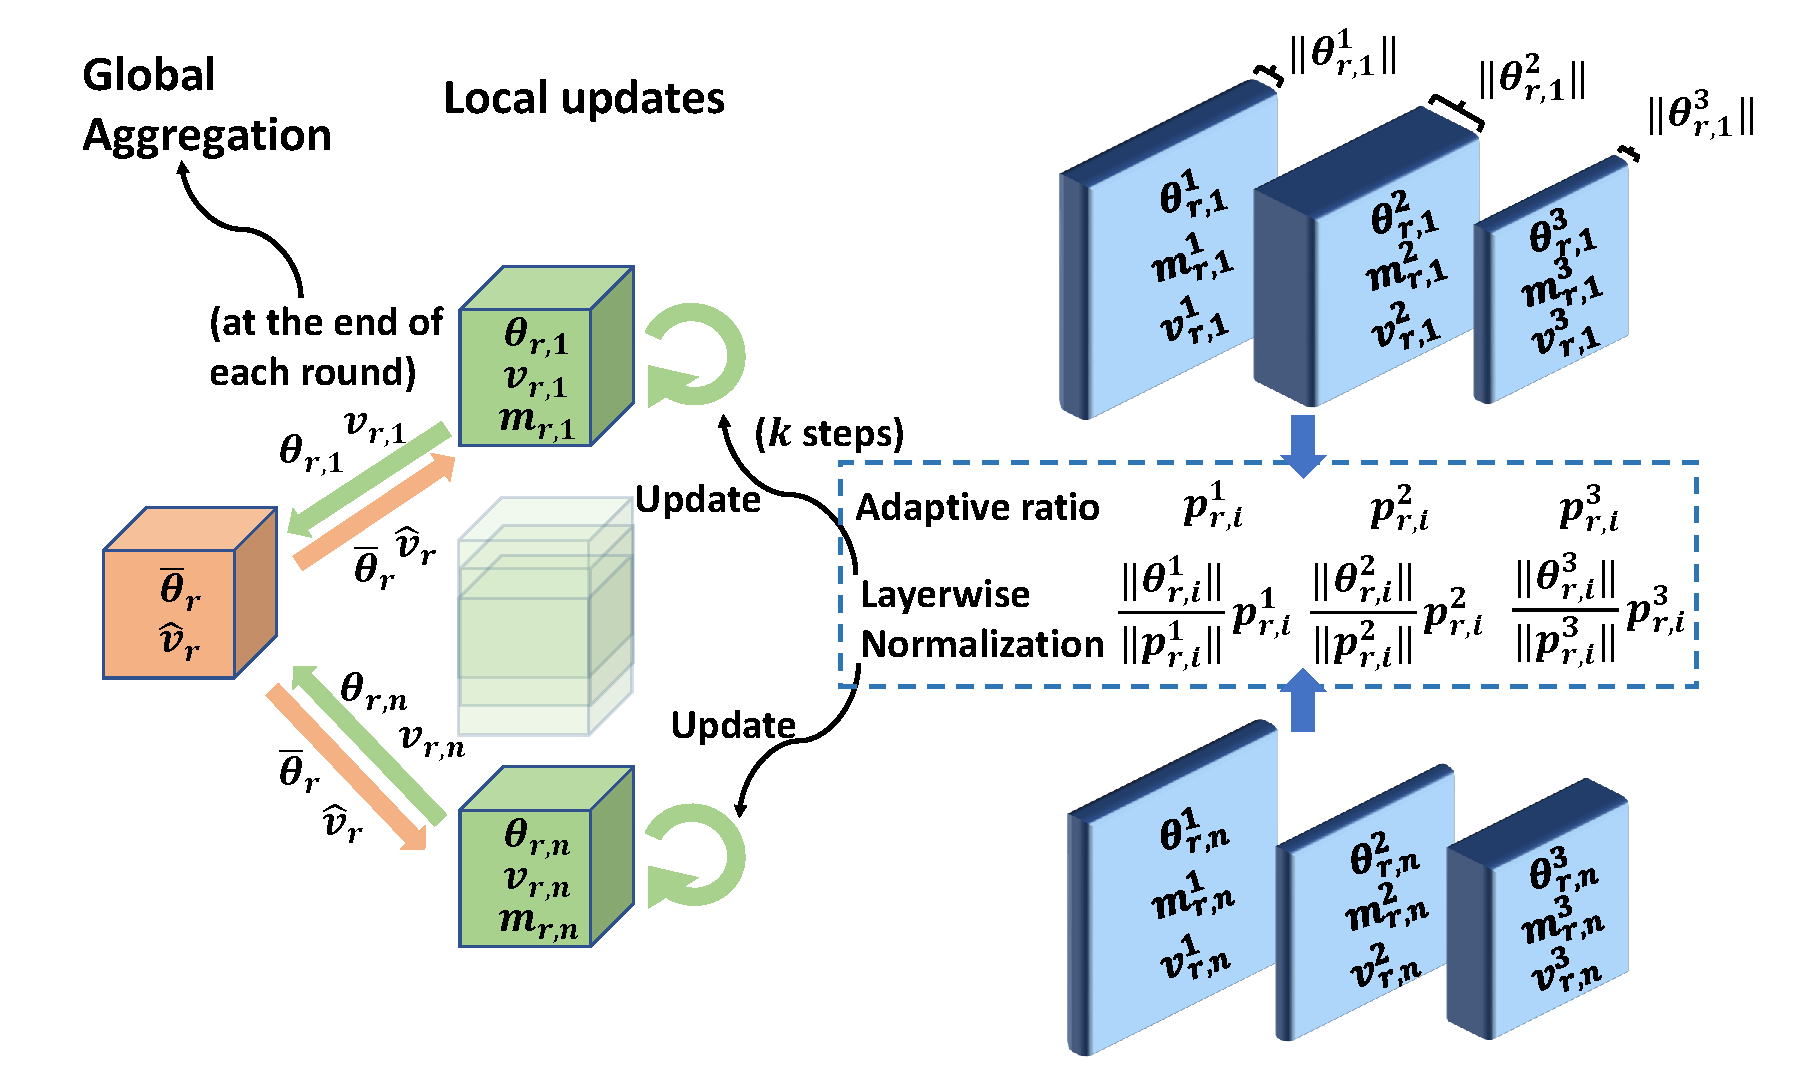
\includegraphics[width=0.8\textwidth]{new_figure/plot1.pdf}
}
\vspace{0.1in}
	\caption{Illustration of \algo\ (Algorithm~\ref{alg:ldams}), with a three-layer network and $\phi(x)=x$ as an example. %	The depth of each network layer represents the norm of its weights. 
		For device $i$ and each local iteration in round $r$, the adaptive ratio of $j$-th layer $p_{r,i}^j$ is normalized according to $\Vert \theta_{r,i}^j\Vert$, and then used for updating the local model. 
	At the end of each round $r$, local worker $i$ sends $\theta_{r,i} =  [\theta_{r,i}^{\ell}]_{\ell =1}^{\tot}$ and $v_{r,i}$ to the central server, which transmits back aggregated $\theta$ and $\hat v$ to local devices to complete a round of training.}
	\label{fig:illustrate}
\end{figure}


\begin{algorithm}[t]
\caption{\algo\ } \label{alg:ldams}
\begin{algorithmic}[1]
%\small
\STATE \textbf{Input}: parameter $0< \beta_1, \beta_2 <1$, and learning rate $\alpha_t$, weight decaying parameter $\lambda \in [0,1]$.
\STATE \textbf{Initialize}: $\theta_{0,i} \in \Theta \subseteq \mathbb R^d $, $m^0_{0,i}=\hat v^0_{0,i}=v^0_{0,i} = 0$, $\forall i\in \llbracket n\rrbracket$, and $\bar{\theta}_0 =  \frac{1}{n} \sum_{i=1}^n \theta_{0,i}$.
\FOR{$r=1$ to $R$}
\FOR{parallel for device $i \in D^{r}$}
\STATE $\qquad$Set $\theta_{r,i}^{0} = \bar{\theta}_{r-1}$.
\STATE $\qquad$Set $m^{0}_{r,i} = m^T_{r-1,i}$\ ,\quad $v^{0}_{r,i} = \hat{v}_{r-1}$.
\FOR{$t=1$ to $T$}
\STATE $\qquad\quad$Compute stochastic gradient $g^t_{r,i}$ at $\theta_{r,i}^{0}$.
\STATE $\qquad\quad$$m^t_{r,i} = \beta_1 m^{t-1}_{r,i} + (1 - \beta_1) g^t_{r,i}$ and $m^{t}_{r,i}=m^{t}_{r,i} /\left(1-\beta_{1}^{t}\right)$. \label{line:new1}
\STATE $\qquad\quad$$v^{t}_{r,i} = \beta_2 v^{t}_{r-1,i} + (1 - \beta_2) (g^t_{r,i})^2$ and $v^{t}_{r,i}=v^{t}_{r,i} /\left(1-\beta_{2}^{t}\right)$. \label{line:new2}
\STATE $\qquad\quad$Compute the ratio  $p_{r,i}^t=m^{t}_{r,i}/(\sqrt{\hat v^{t}_{r}}+\epsilon)$. \label{line:scale}
\STATE $\qquad\quad$Update local model for each layer $\ell \in \llbracket \tot \rrbracket$: \label{line:layer}
\begin{equation}\label{eq:upadtelayer}
    \theta_{r,i}^{\ell,t}=\theta_{r,i}^{\ell,t-1}-\alpha_{r} \phi(\|\theta_{r,i}^{\ell,t-1}\|)(p_{r,i}^{\ell,t}+\lambda \theta_{r,i}^{\ell,t-1})/ \|p_{r,i}^{\ell,t}+\lambda \theta_{r,i}^{\ell,t-1}\|\, .
\end{equation}
\ENDFOR
\STATE $\qquad$Devices send $\theta_{r,i}^{T} = [\theta_{r,i}^{\ell,T}]_{\ell =1}^{\tot}$ and $v_{r,i}^T$ to server.
\ENDFOR
\STATE $\quad$Server computes averages of the local models $\bar{\theta}_r = [\bar{\theta}_r^{\ell,T}]_{\ell =1}^{\tot} = [\frac{1}{n} \sum_{i=1}^n \theta_{r,i}^{\ell,T}]_{\ell =1}^{\tot}$ and $\hat{v}_{r+1} = \max( \hat{v}_{r},\frac{1}{n} \sum_{i=1}^n v^T_{r,i} )$ and send them back to the devices. \label{line:final}
\ENDFOR
\STATE \textbf{Output}: Global model parameter $\bar{\theta}_R = [\bar{\theta}_R^{\ell,T}]_{\ell =1}^{\tot}$.
\end{algorithmic}
\end{algorithm}

For training large deep neural networks, \cite{you2019large} proposed LAMB, an acceleration framework for both SGD and adaptive algorithm that allows large-batch training of BERT in hours. The idea is based on the observation that, during the training of large neural networks, different layers may have very different (absolute) scales, while the magnitude of the gradients in these layers may be similar. Intuitively, this means that in some iterations, the parameter may move a too small step even when the direction (negative gradient) is correct. Therefore, \cite{you2019large} proposed to normalize the gradients in each layer according to the scale of the network layer. Effectively, the algorithm assigns different learning rates to different layers. Empirically, this strategy significantly accelerates the convergence for training large deep models.

Inspired by the merits of local adaptive methods and the success of layer-wise adaptive learning rates, we propose a layer-wise and dimension-wise local AMS algorithm which is detailed in Algorithm~\ref{alg:ldams} and  depicted in Figure~\ref{fig:illustrate}. The proposed algorithm is a natural adaptation of the vanilla AMSGrad method, for multi-layer neural networks under the federated learning setting. Here, ``multi-layer'' includes a broad class of network architectures that can be parameterized layer-by-layer (e.g., CNN, ResNet, Transformers). Lines~8-11 in Algorithm~\ref{alg:ldams} correspond to the standard first and second moment estimation and correction performed by AMSGrad locally. The local model update rule \eqref{eq:upadtelayer} in Line 12 incorporates the layer-wise normalization according to the magnitude of each layer's weights. For example, taking $\phi$ as the identity function and weight decay $\lambda=0$, then the model $\theta$ is updated by $-\frac{\alpha \| \theta\|}{\|p\|}\cdot p$, instead of $-\alpha p$ as in the standard AMSGrad update. The norm of each update is precisely $\alpha \|\theta\|$. That is, we force the change in each layer's parameter to have norm proportional to the scale of the layer's weight. This is a novel extension of the layer-wise adaptivity to the federated learning framework. Therefore, the proposed \algo\ exhibits two-fold adaptivity---a dimension-wise adaptive learning rate with respect to the square root of the second moment used in AMSGrad, and a layer-wise adaptive normalization brought by LAMB. Such two-fold adaptivity has not been considered in FL literature, and we will demonstrate the advantage of this scheme theoretically and empirically in the remainder of the paper.




\section{Convergence of \algo}\label{sec:theory}
In this section, we develop the theoretical analysis of Algorithm~\ref{alg:ldams}.  Based on classical result for stochastic nonconvex optimization, we present a collection of results that aims to providing a better understanding of the convergence behavior of our distributed optimization method under the federated learning framework.
The main challenges we ought to overcome are manifold:
(i) The large amount of decentralized workers working solely on their own data stored locally. 
(ii) A periodic averaging occurs on the central server pushing each of those clients to send local models after some local iterations. 
(iii) Each client computes a backpropagation of the main model, i.e., the deep neural network, and then updates its local version of the model via an adaptive gradient method: the distinctiveness being that those updates are done \emph{dimension-wise} and \emph{layer-wise}.
Our analysis encompasses the consideration of those challenges and leads to an informative convergence rates depending on the quantities of interest in our problem: the number of layers of the DNN, the number of communications rounds and the number of clients used under our federated settings.

\subsection{Finite Time Analysis of \algo}
In the sequel, the analysis of our scheme we provide is \emph{global}, in the sense that it does not depend on the initialization of our algorithm, and \emph{finite-time}, meaning that it is true for any arbitrary number of communication rounds, in particular small ones.
In the particular context of nonconvex stochastic optimization for distributed clients, we assume the following:

\vspace{0.1in}

\begin{assumption}\label{ass:smooth}(Smoothness per layer)
For $i \in \inter$ and $\ell \in \interl$: $\norm{\nabla f_i (\theta^\ell) - \nabla f_i (\vartheta^\ell)} \leq L_\ell \norm{\theta^\ell-\vartheta^\ell}$.
\end{assumption}
We add some classical assumption on the gradient of the objective function:
\begin{assumption}\label{ass:boundgrad}(Unbiased and Bounded gradient)
The stochastic gradient is unbiased for any iteration $r>0$: $\EE[g_r] = \nabla f(\theta_r)$ and is bounded from above, i.e., $\norm{g_t} \leq M$.
\end{assumption}

\begin{assumption}\label{ass:var}(Bounded variance)
The variance of the stochastic gradient is bounded for any iteration $r>0$ and any dimension $j \in \llbracket d \rrbracket$: $\EE[|g_r^j - \nabla f(\theta_r)^j|^2] < \sigma^2$.
\end{assumption}

\begin{assumption}\label{ass:phi}(Bounded Scale)
For any $a \in \rset^*_+$, there exists strictly positive constants such that $\phi_m \leq  \phi(a) \leq \phi_M$.
\end{assumption}



Two important Lemmas are required in the proof of the Theorem above.
We also report the complete proof of our bound in the Appendix of this paper.

The first result gives a characterization of the gap between the averaged model, that is computed by the central server in a periodic manner, and each of the local models stored in each client $i \in \inter$.
\begin{Lemma}\label{lemma:iterates}
Consider $\{\overline{\theta_r}\}_{r>0}$, the sequence of parameters obtained running Algorithm~\ref{alg:ldams}. Then for $i \in \inter$ and $r > 0$, the gap $\| \overline{\theta_r} - \theta_{r,i} \|^2$ satisfies:
\beq\notag
\| \overline{\theta_r} - \theta_{r,i} \|^2 \leq \alpha_r^2 M^2 \phi_M^2 \frac{(1-\beta_2)p}{v_0} \, ,
\eeq
where $\phi_M$ is defined in H\ref{ass:phi} and p is the total number of dimensions $p = \sum_{\ell = 1}^\tot p_\ell$.
\end{Lemma}

The gap is provably bounded by some quantities of interest such as the total dimension of the multi-layered model $p$, the learning rate and the assumed upper bound of the  gradient, see H\ref{ass:boundgrad}.

Note that the end goal is to characterize how fast the gradient of the averaged/global parameter $\overline{\theta_r}$ goes to zero, but not the averaged gradient. The following Lemma allows us to convert the suboptimality condition $\left\| \frac{\overline{\nabla}f(\theta_r)}{\sqrt{ v_r^t}} \right\|$ to the desired one which is $\left\| \frac{\nabla f(\overline{\theta_r})}{\sqrt{ v_r^t}} \right\|$.


\begin{Lemma}\label{lemma:ratio}
Consider $\{\overline{\theta_r}\}_{r>0}$, the sequence of parameters obtained running Algorithm~\ref{alg:ldams}. Then for $r > 0$:
\beq\notag
\left\| \frac{\overline{\nabla}f(\theta_r)}{\sqrt{ v_r^t}} \right\|^2 \geq \frac{1}{2} \left\| \frac{\nabla f(\overline{\theta_r})}{\sqrt{ v_r^t}} \right\|^2 - \overline{L} \alpha^2 M^2 \phi_M^2 \frac{(1-\beta_2)p}{v_0}\, ,
\eeq
where $M$ is defined in H\ref{ass:boundgrad}, $p = \sum_{\ell = 1}^\tot p_\ell$ and $\phi_M$ is defined in H\ref{ass:phi}.
\end{Lemma}


We now state our main result regarding the non asymptotic convergence analysis of our Algorithm~\ref{alg:ldams} for multiple local updates and true for any communication rounds number $R$.



\begin{Theorem}\label{th:multiple update}
Assume \textbf{H\ref{ass:smooth}-H\ref{ass:phi}}. Consider $\{\overline{\theta_r}\}_{r>0}$, the sequence of parameters obtained running Algorithm~\ref{alg:ldams} with a constant learning rate $\alpha$. Let the number of local epochs be $T \geq 1$ and $\lambda = 0$. Then, for any round $R > 0$, we have
\beq \label{bound1multiple}
\begin{split}
&  \frac{1}{R}\sum_{r=1}^R  \EE\left[ \left\| \frac{\nabla f(\overline{\theta_r})}{\hat v_r^{1/4}}   \right \|^2 \right] \leq    \sqrt{\frac{M^2 p}{n}}  \frac{ \triangle}{\tot \alpha R}+4\alpha \left[ \frac{\alpha^2 L}{\sqrt{v_0}} M^2 (T-1)^2 \phi_M^2 (1-\beta_2)p +\phi_M^2\sqrt{M^2+p\sigma^2} \right]  \\
&\hspace{1.5in} +4\alpha \frac{M^2}{\sqrt{v_0}} +      \frac{\phi_M   \sigma^2}{R n} \sqrt{\frac{1 - \beta_2}{M^2 p}  } +4\alpha \left[\phi_M \frac{\tot \sigma^2}{\sqrt{n}}\right]   + cst,
  \end{split}
\eeq
where $\triangle=\EE[f(\bar{\theta}_1)]  - \min \limits_{\theta \in \Theta} f(\theta)$.
\end{Theorem}

By choosing a suitable decreasing learning rate, we have the following simplified result.
\begin{Corollary}\label{coro:main}
Under the same setting as Theorem~\ref{th:multiple update}, with $\alpha = \mathcal{O}(\frac{1}{ \sqrt{\tot R}})$, it holds that
\begin{align} \label{coro:rate}
\frac{1}{R}\sum_{r=1}^R  \EE\left[ \left\| \frac{\nabla f(\overline{\theta_r})}{\hat v_t^{1/4}}   \right \|^2 \right]\leq \mathcal{O}\left( \sqrt{\frac{ p}{n}} \frac{1}{\sqrt{\tot R}} + \frac{\sigma^2 }{R n\sqrt{p}}+\frac{(T-1)^2p}{\tot^3 R^{3/2}}\right).
\end{align}
\end{Corollary}

The leading two terms display a dependence of the convergence rate of \algo\ on the initialization and the variance of the stochastic gradient (see H\ref{ass:var}), which are common in distributed optimization. The last term involves the number of local updates which relates to the communication efficiency. More discussion will be provided next.

%We recall that a $\epsilon-$stationary point is defined by the number of communication rounds $R$ such that $\frac{1}{R}\sum_{t=1}^\mathcal{R}  \EE\left[ \left\| \frac{\nabla f(\overline{\theta_t})}{\hat v_t^{1/4}}   \right \|^2 \right] \leq \epsilon$.


%\begin{Theorem}\label{th:main}
%Assume \textbf{H\ref{ass:smooth}-H\ref{ass:phi}}. Consider $\{\overline{\theta_r}\}_{r>0}$, the sequence of parameters obtained via Algorithm~\ref{alg:ldams} with a decreasing lr $\alpha_r$. Then, if $T=1$ and $\lambda = 0$:
%%\beq \label{bound1}
%%\begin{split}
%%  \frac{1}{R}\sum_{r=1}^R  \EE\left[ \left\| \frac{\nabla f(\overline{\theta_r})}{\sqrt{ v_r^t}}   \right \|^2 \right] 
%%   \leq &  \sqrt{\frac{M^2 p}{n}} \frac{ \EE[f(\bar{\theta}_1)]  - \min \limits_{\theta \in \Theta} f(\theta)}{\tot \alpha_r R}+      \frac{\phi_M   \sigma^2}{R n} \sqrt{\frac{1 - \beta_2}{M^2 p}  } \\
%%  +& \alpha_r \phi_M \sigma \tot p \sqrt{n}+ \frac{ \overline{L}\beta_1^2\tot(1-\beta_2)M^2 \phi^2_M n}{2(1-\beta_1)^2 v_0}    \\
%% + &\frac{\alpha_r \beta_1}{1-\beta_1}  \sqrt{(1-\beta_2)p} \frac{\tot M^2}{\sqrt{v_0}} +\overline{L} \alpha_r^2 M^2 \phi_M^2 \frac{(1-\beta_2)p}{Rv_0} 
%%   \end{split}
%%\eeq
%\beq \label{bound1}
%\begin{split}
%  \frac{1}{R}\sum_{r=1}^R  \EE\left[ \left\| \frac{\nabla f(\overline{\theta_r})}{\sqrt{ v_r^t}}   \right \|^2 \right] 
%   \leq   \sqrt{\frac{M^2 p}{n}} \frac{ \EE[f(\bar{\theta}_1)]  - f^*}{\tot \alpha_r R} + \frac{\phi_M}{R} \left[ \frac{(1-\beta_2)\overline{L} \alpha_r^2 M^2 \phi_Mp}{v_0} +  \frac{ \sigma^2}{n} \sqrt{\frac{1 - \beta_2}{M^2 p}  }    \right]
%   \end{split}
%\eeq
%where $\overline{L} = \sum_{\ell=1}^\tot L_{\ell}$ is the sum of all smoothness constants, $\tot$ is the total number of layers and $f^* \eqdef \min \limits_{\theta \in \Theta} f(\theta)$.
%\end{Theorem}


\subsection{Comparisons}

We dedicate the following paragraph to a discussion on the bound (and implications) derived above in comparison with known results most relevant to our interest in literature.

\vspace{0.1in}
\noindent\textbf{LAMB bound in~\citet{you2019large}: }
We first start our discussion with the comparison of convergence rate of \algo\ with that of LAMB, Theorem 3 in~\citet{you2019large}. 
The convergence rates of \algo and LAMB differ in two ways: 
(i) First, note that the characterization, on the suboptimality, or convergence criterion, is given at the averaged parameters noted $\overline{\theta}_r$ due to our distributed settings. 
It is thus natural to consider the evolution of our objective function, precisely its gradient, evaluated at some global model values --as opposed to the outcome of a single step drift in the central server paradigm. 
Besides, for ease of interpretation, the LHS of~\eqref{bound1multiple} is summed over all rounds instead of a fictive random termination point. A simple calculation would lead to such characterization found in several nonconvex stochastic optimization paper such as~\cite{ghadimi2013stochastic}.
(ii) Assuming that the convergence criterion in both Theorems is of similar order (which happens for a large enough number of rounds), the convergence rate of \algo\ displays a similar $\mathcal{O}(1/R)$ behaviour for the initialization term. That said, despite the distributed (federated) setting, our dimension-wise and layer-wise method benefits from the double adaptivity phenomenon explained above and exhibited in LAMB~\citep{you2019large}, under a central server setting.


\vspace{0.1in}
\noindent\textbf{Fed-AMS bound in~\citet{chen2020toward}: }
We now discuss the similarities and differences between Fed-AMS, the baseline distributed adaptive method developed in~\citet{chen2020toward}, and our \algo. For clarity, we restate their main result (Theorem~\ref{thm:chen}) under our notations.

\begin{Theorem}[Corollary 5.2 in~\citet{chen2020toward}]  \label{thm:chen}
Under some regularity conditions on the local losses and similar assumption as ours, with some properly chosen learning rate, when $R\geq \mathcal O(T^3\sqrt n)$, Fed-AMS has convergence rate
\beq \label{eqn:chen rate}
\begin{split}
 \frac{1}{R}\sum_{r=1}^R  \EE\left[ \left\| \frac{\nabla f(\overline{\theta_r})}{\sqrt{ v_r}}   \right \|^2 \right]     \leq  \mathcal O( \frac{\sqrt p}{\sqrt{n R}}).
 \end{split}
\eeq
\end{Theorem}

\vspace{0.2in}

Firstly, when the number of rounds $R$ is sufficiently large, both rates \eqref{coro:rate} and \eqref{eqn:chen rate} are dominated by $\mathcal O(\frac{\sqrt p}{\sqrt{n R}})$, matching the convergence rate of the standard AMSGrad (e.g.~\cite{Arxiv:Zhou_18}).
The acceleration of our layer-wise scheme is exhibited in the $\mathcal O(1/(n R))$ term and the dependence on the number of layers $\mathcal O(1/(h^3 R^{3/2}))$ term. Note that the boundedness assumption is on each dimension in H\ref{ass:var} and leads to a manifestation of the term $\sqrt{p}$ in both rates. This dependency on $p$ can be removed when H\ref{ass:var} is assumed globally, which is also common in optimization literature.

Secondly, in~\eqref{coro:rate}, the last term containing the number of local updates $T$ is small as long as $T\leq \mathcal O(\frac{R^{1/2}h^{5/4}}{(np)^{1/4}})$. 
Treating $p^{1/4}/h=\mathcal O(1)$, the result implies that for a given $T$, we can get the same rate of convergence as vanilla AMSGrad with $R\geq \mathcal{O}(T^2\sqrt n)$ rounds of communication. From Theorem~\ref{thm:chen}, we know that Fed-AMS requires $R\geq \mathcal O(T^3\sqrt n)$ rounds to achieve the same rate. This implies that, our \algo\ reduces the number of communication rounds needed to reach an $\epsilon$-stationary point compared with~\cite{chen2020toward}. Therefore, by leveraging the layer-wise acceleration on local models, our \algo\ improve the communication cost of Fed-AMS.


\vspace{0.1in}

\subsection{More Discussion}

We provide more discussion on the algorithmic and theoretical properties of \algo\ from the following aspects:


\vspace{0.1in}
\noindent\textbf{Communication and Client Efficiency:} The (sublinear) dependence on the number of communication rounds of our bound matches that of most recent methods in federated learning, e.g. SCAFFOLD~\citep{karimireddy2019scaffold}, a solution to the problem posed by heterogeneity of the data in each client. Yet, contrary to SCAFFOLD, our method only sends bits once per communication round while SCAFFOLD needs to send two vectors, including an additional control variate term  from the clients to the central server. Our result also matches the communication bound of~\cite{reddi2020adaptive} which adapts Adam~\citep{KB15} to the federated setting. However, the algorithm of~\cite{reddi2020adaptive} performs adaptive updates only at the central server, while SGD is still used for local updates. In addition, the $1/\sqrt n$ term in convergence rate of \algo\ implies a linear speedup effect in the number of local workers, which also matches the dependency on $n$ of most federated learning methods. 


\vspace{0.1in}
\noindent\textbf{Data Heterogeneity:} To demonstrate the effect of non-iid data distribution theoretically, some related works pose assumptions on the global variance and the local variance of the stochastic gradients of the objective function~\eqref{eq:opt} separately, such that both variances appears in the convergence rate. Our analysis can also be easily extended to incorporate the global variance term. While some works including~\citet{karimireddy2019scaffold} target on designing specific strategies to alleviate the negative influence of data heterogeneity, we note that our \algo\ are, in some sense, naturally capable of balancing the heterogeneity in different local data distributions. As mentioned before, this is largely due to the ``moment averaging'' step (line 16 in Algorithm~\ref{alg:ldams}), where the adaptive learning rates guided by the second moment estimation are aggregated among local workers periodically. In our experiments, we will see that the advantage of \algo\ is consistent under both homogeneous and heterogeneous data setting. 

% \medskip
% \textbf{Dependence on the dimension $p$:} The $\sqrt p$ term appearing in our bound is due to the assumption on coordinate-wise bounded variance. One may instead assume a bounded total variance to remove this term. 
% In practice, the dependence on the overall size of the vectors being transmitted back and forth from the central to the devices can be improved in various ways. Indeed, recent efficient techniques aim at reducing the number of bits communicated at each round through sketches or compression techniques, see for instance~\citet{haddadpour2020fedsketch,ivkin2019communication,li2019privacy} to name a few.
% This can be a great addition to \algo, and is naturally compatible, but is not the main focus of our contribution.




\section{Numerical Experiments}\label{sec:numerical}

In this section, we conduct numerical experiments on various datasets and network architectures to justify the effectiveness of our proposed method in practice. Our main objective is to validate the benefit of dimension-wise adaptive learning when integrated with the locally adaptive FL method.
We observe that our method empirically confirms its edge in terms of convergence speed.
Basically, \algo\ reduces the number of rounds and thus the communication cost required to achieve a similar stationary point (or test accuracy) than the baseline methods. In many cases, \algo\ could also bring notable improvement in the generalization performance.


\vspace{0.1in}
\noindent\textbf{Methods and tuning.} In our experiments, we evaluate four federated learning algorithms: 
\begin{enumerate}
    \item Fed-SGD~\citep{mcmahan2017communication}, standard federated averaging with local SGD updates.
    
    \item Fed-AMS~\citep{chen2020toward}, locally adaptive AMSGrad.
    
    \item Adp-Fed (``Adaptive Federated Optimization''), the federated adaptive algorithm proposed by~\cite{reddi2020adaptive}. The algorithm performs local SGD updates. At the end of each round $r$, the changes in local models, $\triangle_i=w_{r,i}^T-w_{r,i}^0$, $i=1,...,n$, are transformed to the central server for an aggregated Adam update. See Appendix~\ref{app:experiment} for a precise algorithm description.
    
    \item Our proposed \algo\ (Algorithm~\ref{alg:ldams}), layer-wise accelerated local AMSGrad.
\end{enumerate}
For all the adaptive methods, we set hyper-parameters $\beta_1=0.9$, $\beta_2=0.999$ as the recommended default~\citep{reddi2019convergence}. Regarding the federated learning environment, we use 50 local workers with 0.5 participation rate. That is, we randomly pick half of the workers to be active for training in each round. We set the local mini-batch size as 128. In each round, the training samples are allocated to the active devices, and one local epoch is finished after all the local devices run one epoch over their received samples by mini-batch training. 

We tune the initial learning rate $\alpha$ for each algorithm over a fine grid. For Adp-Fed, there are two learning rates involved. We tune the combination of local learning rate (for local SGD) and global learning rate (for global Adam) over a fine grid. For \algo\, the parameter $\lambda$ in Algorithm~\ref{alg:ldams} controlling the overall scale of the layer-wise gradients is tuned from $\{0,0.01,0.1\}$, and use the identity function for $\phi(\cdot)$. The detailed parameter tuning diagram can be found in Appendix~\ref{app:experiment}.
For each run, we report the test accuracy with the best $\alpha$ and $\lambda$. The results are averaged over three independent runs, each with same initialization for every method.

\vspace{0.1in}
\noindent\textbf{Datasets and models.} We run our experiments on four popular benchmark image classification datasets: MNIST~\citep{lecun1998mnist}, Fashion MNIST (FMNIST)~\citep{xiao2017fashion}, CIFAR-10~\citep{krizhevsky2009learning} and TinyImageNet~\citep{deng2009imagenet}. The MNIST dataset contains 60000 training samples and 10000 test samples, from 10 classes of handwritten digits from 0 to 9. The FMNIST dataset has the same sample size and train/test split as MNIST, but the samples are fashion products (e.g., dress, bags) which makes it harder to train than MNIST. The CIFAR-10 dataset has 50000 training images and 10000 test images, from 10 classes. The TinyImageNet is a subset of the ImageNet dataset. It includes 100000 $64\times 64$ images for from 200 classes for training and 10000 for testing. For MNIST, we apply 1) a simple multi-layer perceptron (MLP), which has one hidden layer containing 200 cells with dropout; 2) Convolutional Neural Network (CNN), which has two max-pooled convolutional layers followed by a dropout layer and two fully-connected layers with 320 and 50 cells respectively. This CNN is also implemented for FMNIST. For CIFAR-10 and TinyImageNet, we implement ResNet-18 network~\cite{Proc:He-resnet16}.


\subsection{Comparison under iid setting}

In Figure~\ref{fig:iid}, we report the test accuracy of MLP trained on MNIST, as well as CNN trained on MNIST and FMNIST, where the data is i.i.d. allocated among the clients. We test 1 local epoch and 3 local epochs (more local iterations). In all the figures, we observe a clear advantage of \algo\ over the competing methods in terms of the convergence speed. In particular, we can see that \algo\ is able to achieve the same accuracy with fewest number of communication rounds, thus improving the communication efficiency. For instance, this can be observed as follows: on MNIST + CNN (1 local epoch), Fed-AMS requires 20 rounds to achieves 90\% accuracy, while \algo\ only takes 5 rounds. This implies a 75\% reduction in the communication cost. Moreover, on MNIST, \algo\ also leads to improved generalisation performance, i.e., test accuracy. Note that, the result on MLP to a good extent provides a straightforward illustration on the benefit of layer-wise adaptivity in \algo\, since compared with Fed-AMS, the only difference is that the learning rate becomes adaptive to the scale of the single hidden layer in \algo. Lastly, we see a faster convergence with 3 local epochs. For iid data distribution, this is expected and consistent with previous results in literature (e.g., \cite{reddi2020adaptive}).


\begin{figure}[h]
    \begin{center}
        \mbox{
        \hspace{-0.1in}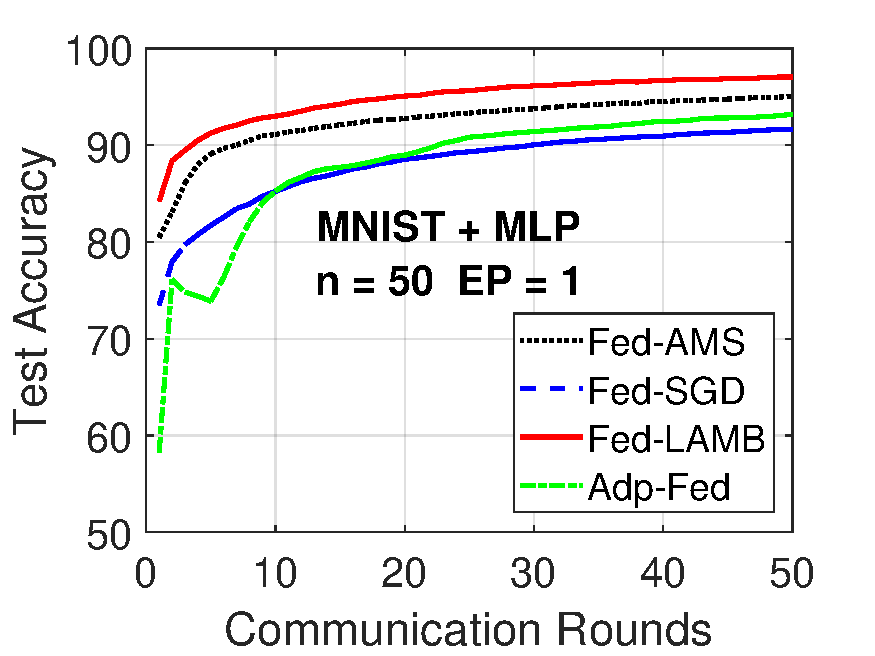
\includegraphics[width=0.35\textwidth]{new_fmnist_mnist_fig/mnist_testerror_mlp_ep1_iid1_reddi.pdf}
        \hspace{-0.1in}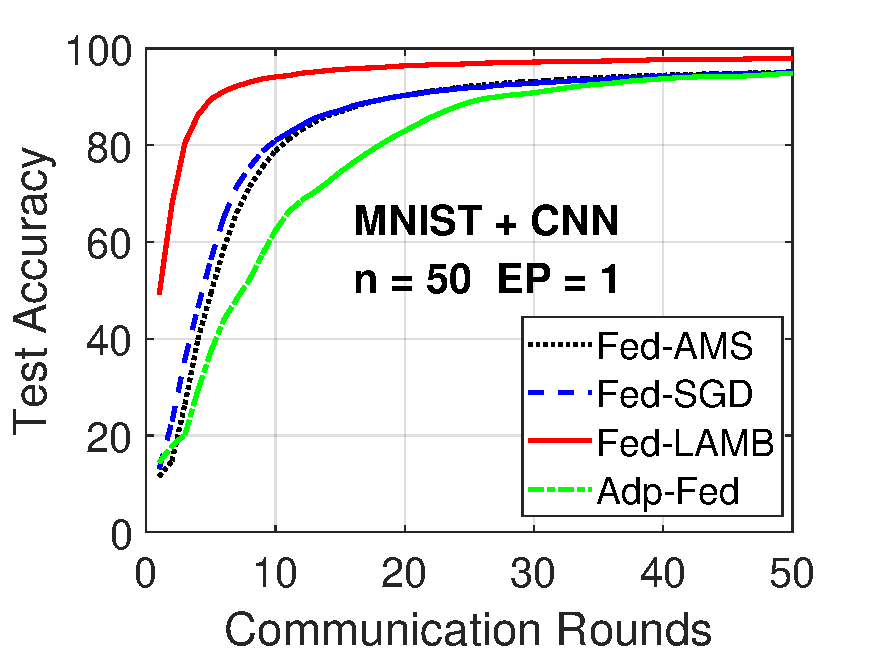
\includegraphics[width=0.35\textwidth]{new_fmnist_mnist_fig/mnist_testerror_cnn_ep1_iid1_reddi.pdf}
        \hspace{-0.1in}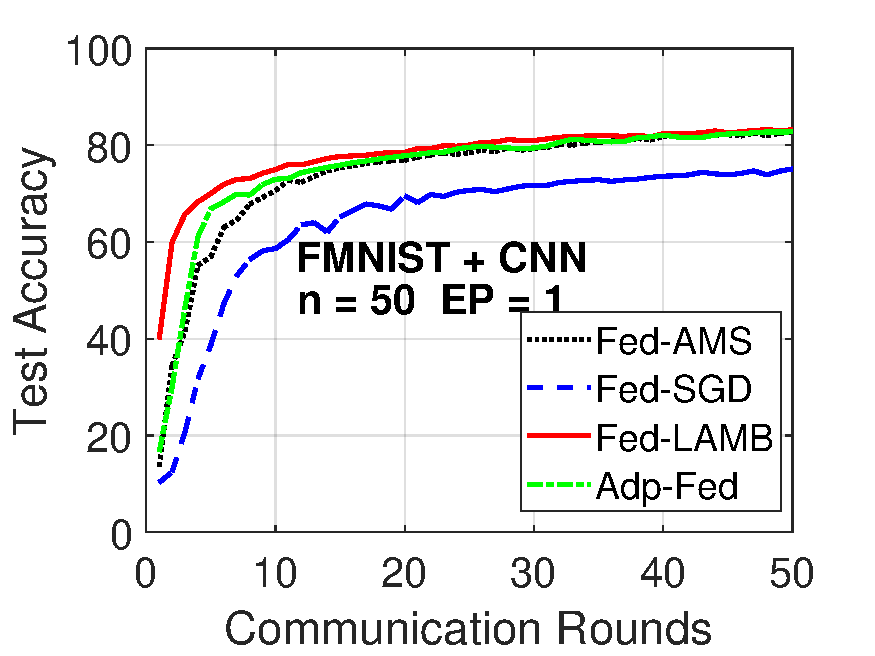
\includegraphics[width=0.35\textwidth]{new_fmnist_mnist_fig/fmnist_testerror_cnn_ep1_iid1_reddi.pdf}
        }
        \mbox{
        \hspace{-0.1in}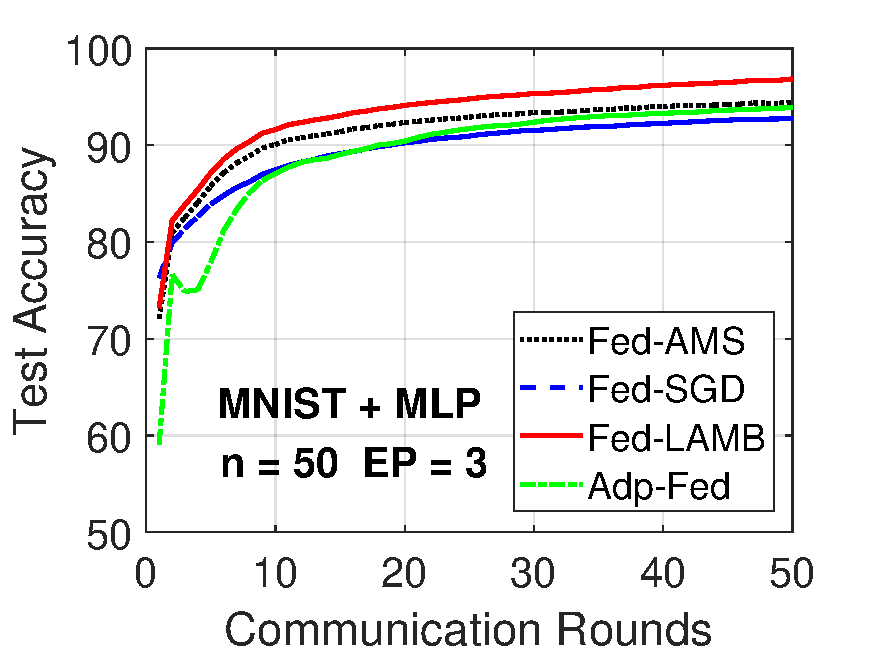
\includegraphics[width=0.35\textwidth]{new_fmnist_mnist_fig/mnist_testerror_mlp_ep3_iid1_reddi.pdf}
        \hspace{-0.1in}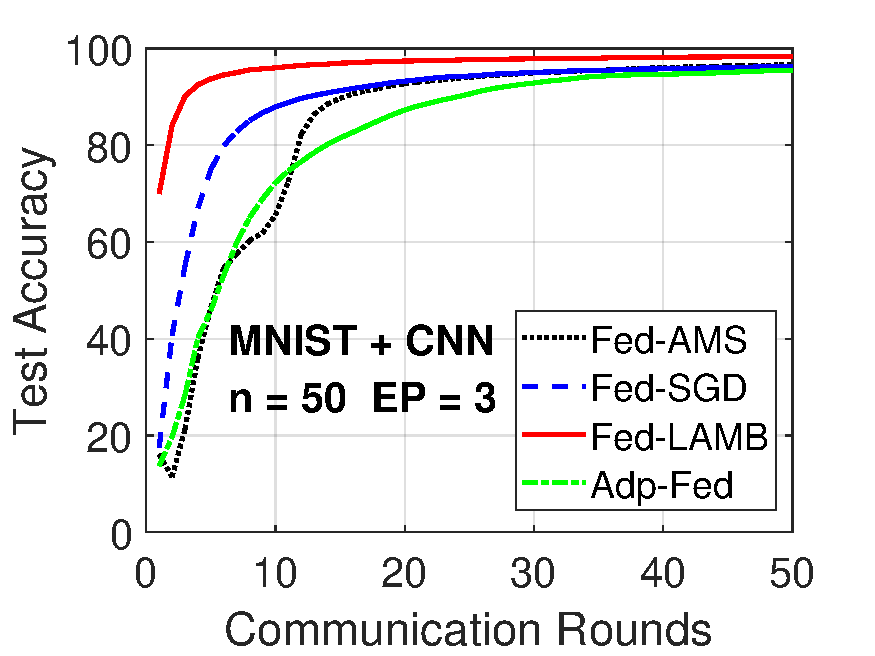
\includegraphics[width=0.35\textwidth]{new_fmnist_mnist_fig/mnist_testerror_cnn_ep3_iid1_reddi.pdf}
        \hspace{-0.1in}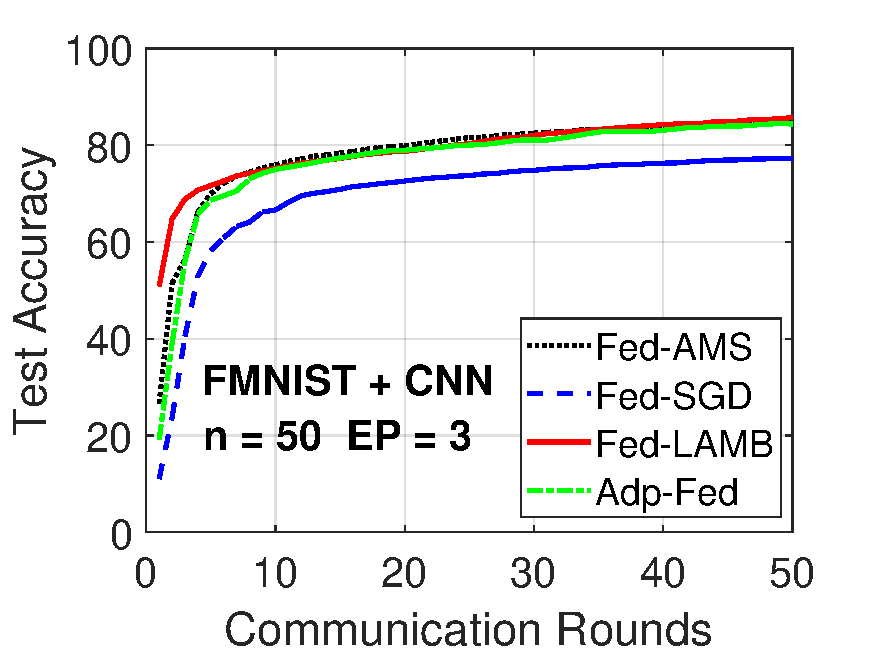
\includegraphics[width=0.35\textwidth]{new_fmnist_mnist_fig/fmnist_testerror_cnn_ep3_iid1_reddi.pdf}
        }
    \end{center}
	\caption{\textbf{i.i.d. data setting}. Test accuracy on MNIST and FMNIST against the number of communication rounds with 50 clients. \textbf{1st row:} 1 local epoch. \textbf{2nd row:} 3 local epochs. We see that \algo\ converges faster to better solution (higher test accuracy) in all cases.
	}
	\label{fig:iid}\vspace{-0.1in}
\end{figure}


\subsection{Comparison under non-iid setting}



In Figure~\ref{fig:noniid}, we provide the results on  MNIST and FMNIST dataset, when the local data has non-iid distribution (i.e., under data heterogeneity). In particular, in each round of federated training, every local device only receives samples from one class (out of ten). This is known to be the scenario where federated learning is harder to generalize well~\citep{mcmahan2017communication}, thus an important case for the empirical evaluation of FL methods. 

First of all, from Figure~\ref{fig:noniid}, we see that for experiments with 1 local epoch, in all cases our proposed \algo\ outperforms the three baseline methods. Similar to the plots for iid data setting, \algo\ provides faster convergence speed and achieves higher test accuracy than Fed-SGD and Fed-AMS. The advantage is especially significant for the CNN model, e.g., it improves the accuracy of Fed-SGD and Fed-AMS by more than 10\% on FMNIST. On both two datasets, \algo\ saves around 50\% communication rounds to reach a same accuracy level as Fed-AMS. The other baseline method, Adp-Fed, performs as good as our \algo\ on FMNIST, but worse than other methods on MNIST.

The relative comparison is basically the same when we conduct 3 local epochs. Yet, the advantage of \algo\ becomes less significant than what we observed in Figure~\ref{fig:iid} with iid local data distribution. One plausible reason is that when the local data is highly non-iid as in our case, the fast convergence of the local models as in \algo\ might not be as beneficial when we allow too many local updates per round. Intuitively speaking, learning the local models ``too fast'' might not be a good thing to the globally aggregated model, since each local model is trained only with a few classes of data points, i.e., local models target at different loss functions.



\begin{figure}[t]
    \begin{center}
        \mbox{
        \hspace{-0.1in}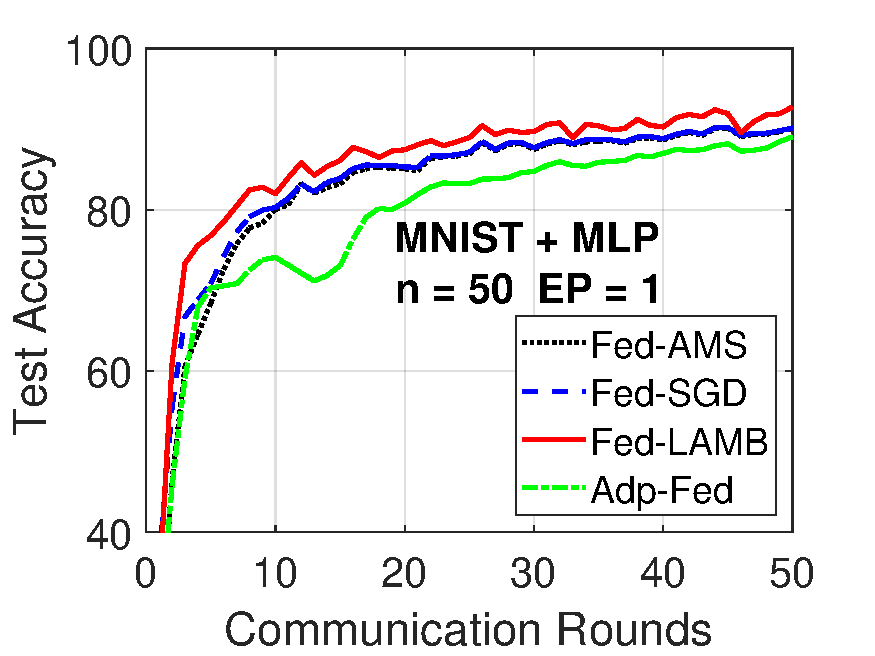
\includegraphics[width=0.35\textwidth]{new_fmnist_mnist_fig/mnist_testerror_mlp_ep1_iid0_reddi.pdf}
        \hspace{-0.1in}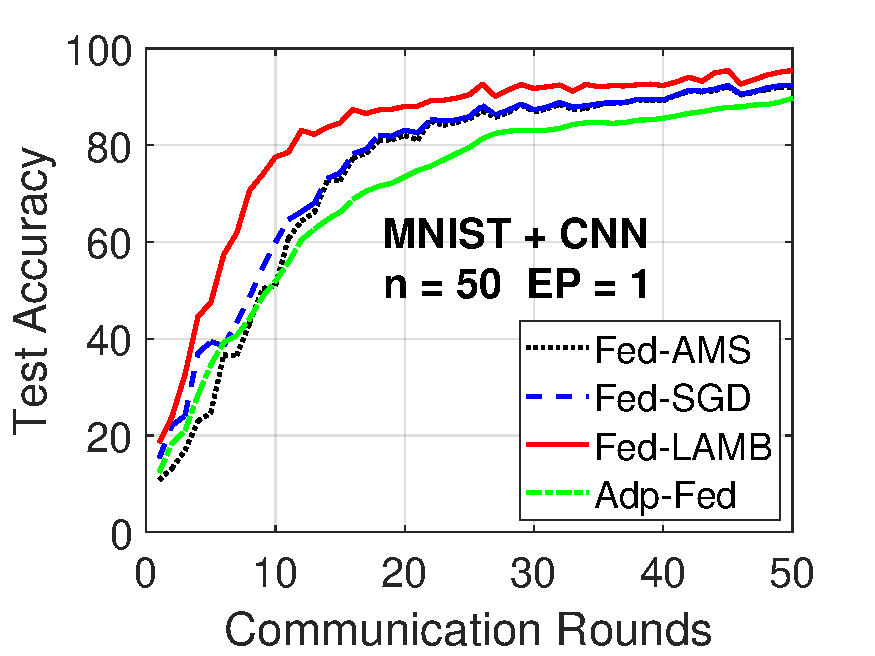
\includegraphics[width=0.35\textwidth]{new_fmnist_mnist_fig/mnist_testerror_cnn_ep1_iid0_reddi.pdf}
        \hspace{-0.1in}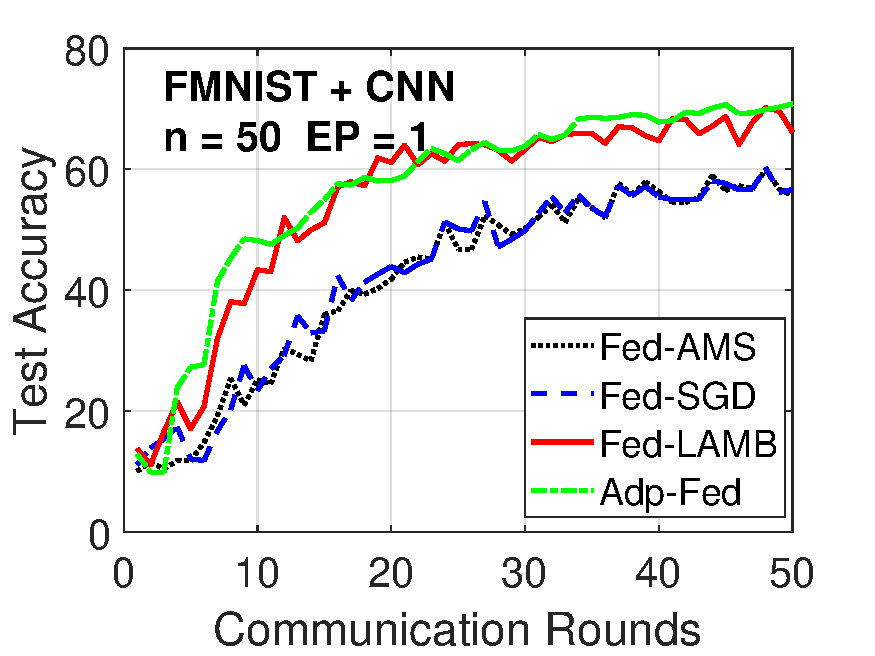
\includegraphics[width=0.35\textwidth]{new_fmnist_mnist_fig/fmnist_testerror_cnn_ep1_iid0_reddi.pdf}
        }
        \mbox{
        \hspace{-0.1in}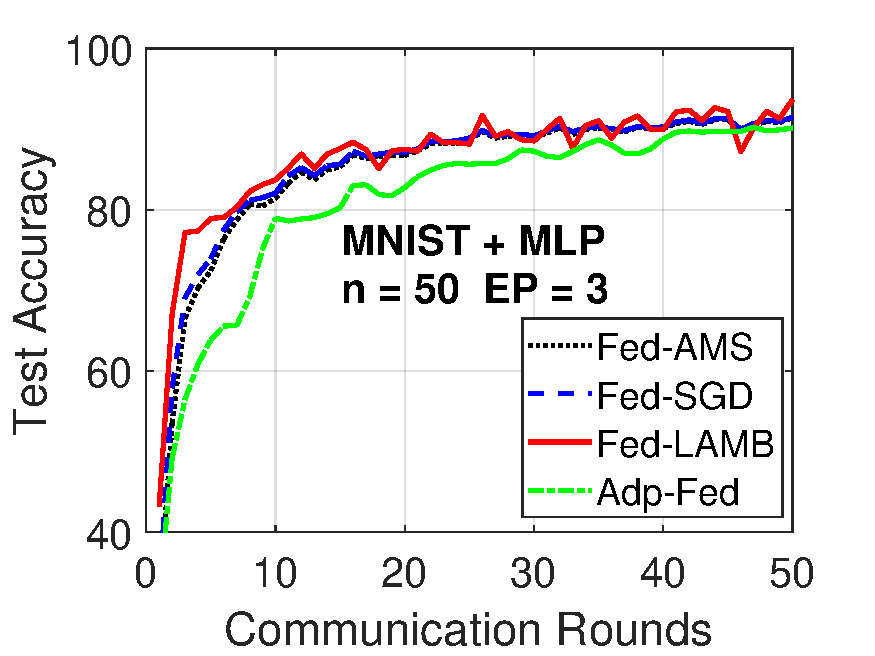
\includegraphics[width=0.35\textwidth]{new_fmnist_mnist_fig/mnist_testerror_mlp_ep3_iid0_reddi.pdf}
        \hspace{-0.1in}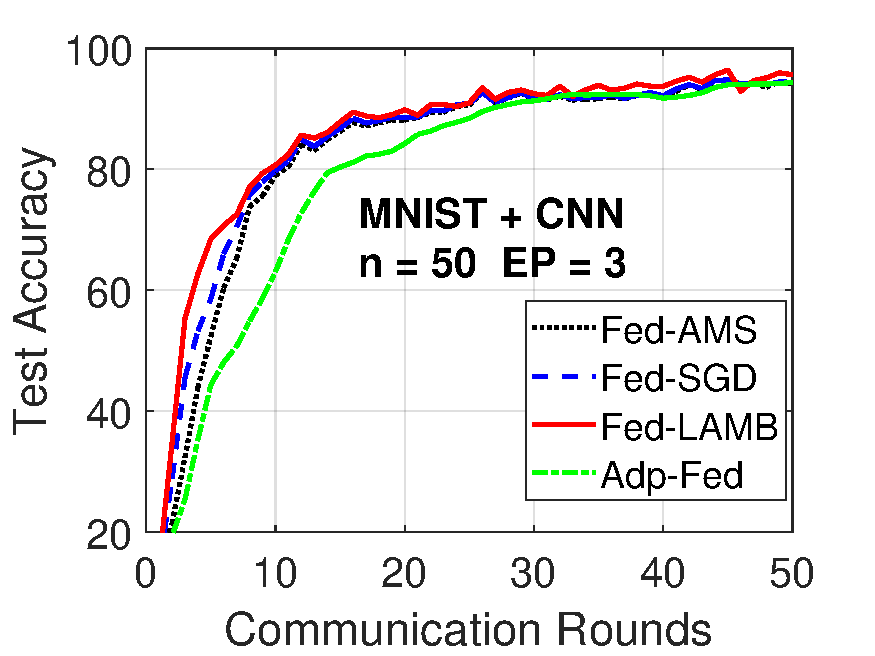
\includegraphics[width=0.35\textwidth]{new_fmnist_mnist_fig/mnist_testerror_cnn_ep3_iid0_reddi.pdf}
        \hspace{-0.1in}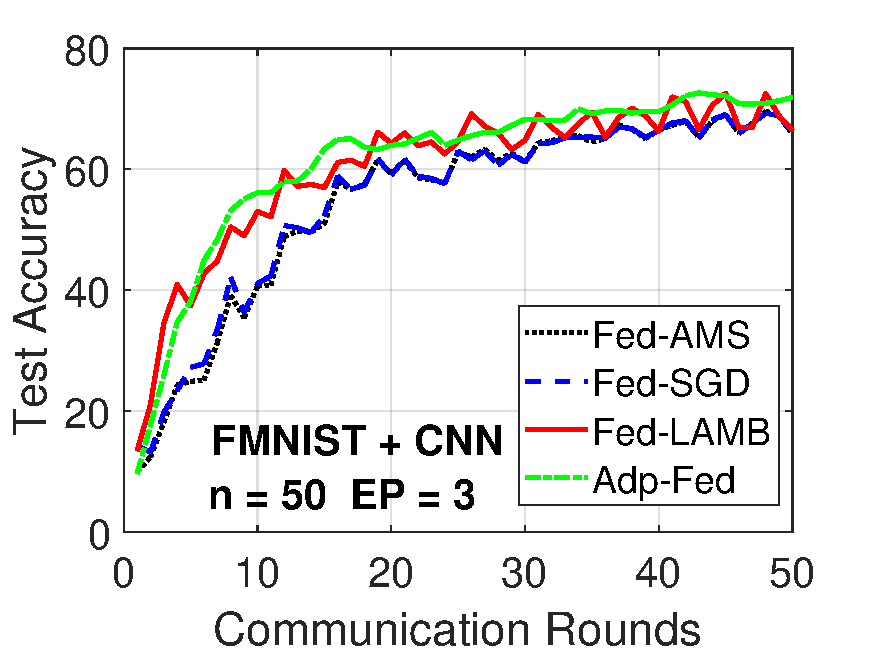
\includegraphics[width=0.35\textwidth]{new_fmnist_mnist_fig/fmnist_testerror_cnn_ep3_iid0_reddi.pdf}
        }
        % \mbox{
        % \hspace{-0.05in}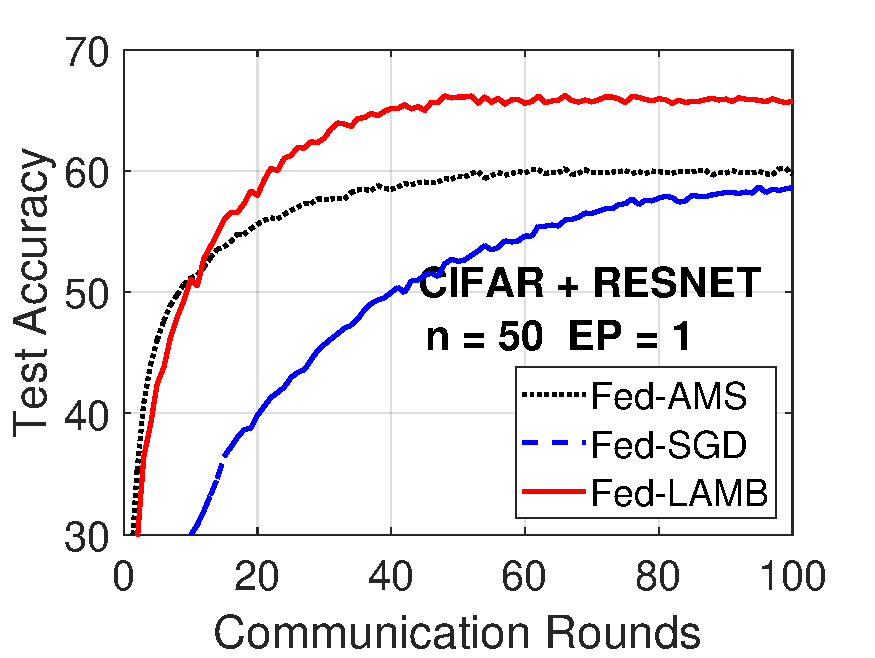
\includegraphics[width=0.25\textwidth]{new_figure/cifar_testerror_resnet_ep1_client50_iid0.pdf}
        % \hspace{-0.1in}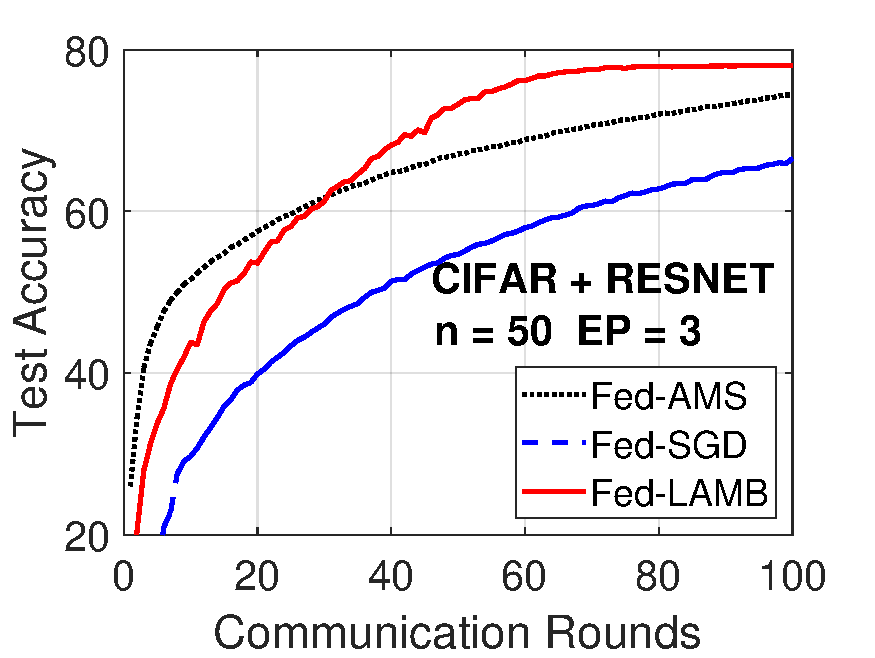
\includegraphics[width=0.25\textwidth]{new_figure/cifar_testerror_resnet_ep3_client50_iid0.pdf}        
        % }
    \end{center}
	\caption{\textbf{non-i.i.d. data setting.} Test accuracy on MNIST and FMNIST against the number of communication rounds, with 50 clients. \textbf{1st row:} 1 local epoch. \textbf{2nd row:} 3 local epochs. We see that \algo\ converges faster to better solution (higher test accuracy) in all cases.}
	\label{fig:noniid}
%	\vspace{-0.5in}
\end{figure}

\clearpage

In Figure~\ref{fig:noniidresnet18}, we present the experiment results on CIFAR-10 and TinyImageNet datasets trained by ResNet-18. When training these two models, we decrease the learning rate by 10 at 30 and 70 communication rounds. From Figure~\ref{fig:noniidresnet18}, we can draw similar conclusion as before: the proposed \algo\ is the best method in terms of both convergence speed and generalization accuracy. In particular, on TinyImageNet, we see that \algo\ has a significant advantage over all three baselines. Although Adp-Fed performs better than Fed-SGD and Fed-AMS, it is considerably worse than \algo. For reference, we also report the overall test accuracy at the end of training in Table~\ref{tab:acc}. \algo\ achieves the highest accuracy on both datasets. On TinyImagenet, \algo\ reaches $76\%$ after 100 communication rounds, against around $65\%$ for Fed-AMS, $68\%$ for Fed-SGD and $74\%$ for Adp-Fed.


\begin{figure}[t]
\vspace{-0.15in}
    \begin{center}
        \mbox{
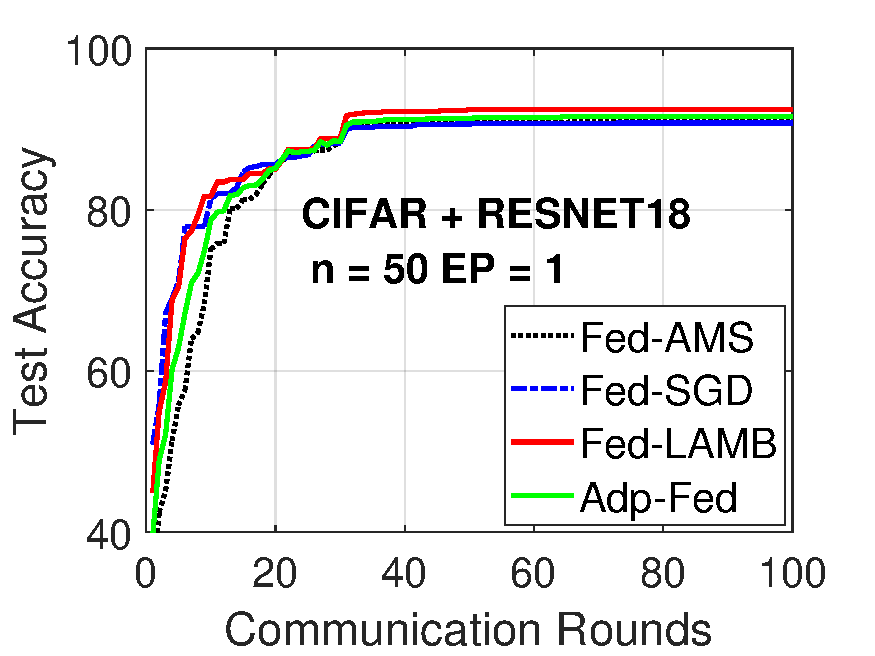
\includegraphics[width=0.4\textwidth]{new_fmnist_mnist_fig/cifar_testerror_resnet18_ep1_client2_iid0_reddi.pdf}
        \hspace{-0.1in}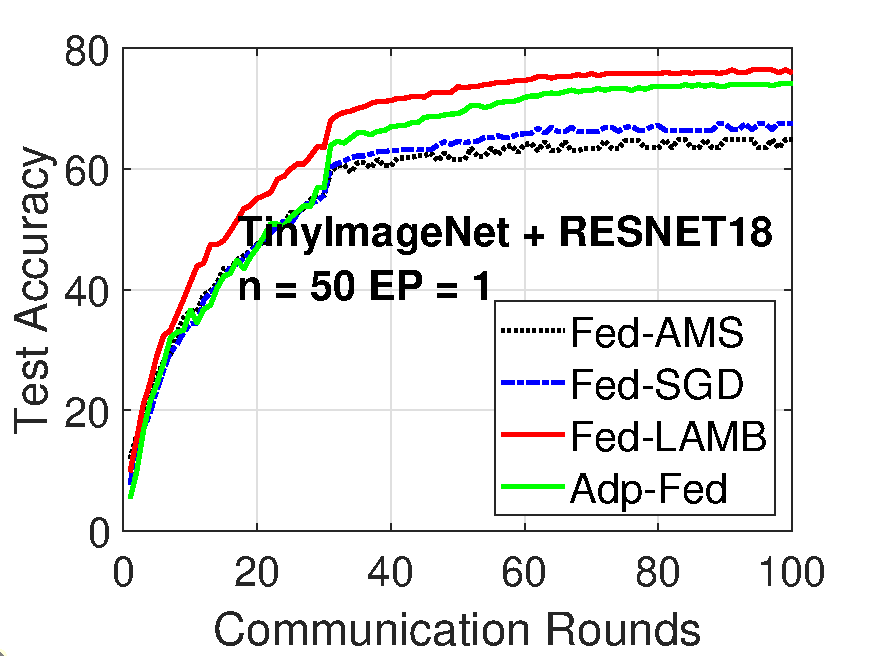
\includegraphics[width=0.4\textwidth]{new_fmnist_mnist_fig/tinyimagenet_testerror_resnet18_ep1_client2_iid0_reddi.pdf}\hspace{-0.1in}
        % \includegraphics[width=0.4\textwidth]{new_figure/tinyimagenet_testerror_resnet18_ep1_client2_iid0.eps}
        }
    \end{center}
	\caption{\textbf{non-i.i.d. data setting.} Test accuracy on CIFAR-10 + ResNet-18 and TinyImagenet + ResNet-18 with 50 clients.
	}
	\label{fig:noniidresnet18}\vspace{-0.1in}
\end{figure}

\begin{table}[h]
\centering
\caption{Test Accuracy on ResNet-18 Network.}\label{tab:acc}
	\resizebox{0.9\columnwidth}{!}{%
\begin{tabular}{lllll}
\toprule[1pt]
 & Fed-SGD      & Fed-AMS    & Adp-Fed     & \textbf{\algo\ }       \\ \hline
CIFAR-10 & 90.75 $\pm$ 0.48  & 90.93 $\pm$ 0.22 & 91.57 $\pm$ 0.38  & 92.44 $\pm$ 0.53 \\
% TinyImageNet & 79.64 $\pm$ 0.21  & 75.94 $\pm$ 0.83  & 93.50 $\pm$ 0.26 \\
TinyImageNet & 67.58 $\pm$ 0.21  & 64.86 $\pm$ 0.83 & 74.17 $\pm$ 0.43  & 76.00 $\pm$ 0.26 \\
\toprule[1pt]
\end{tabular}
}\vspace{-0.2in}
\end{table}



\section{Conclusion}\label{sec:conclusion}

We study a doubly adaptive method in the particular framework of federated learning.
Built upon the success of periodic averaging, and of state-of-the-art adaptive gradient methods for single server nonconvex stochastic optimization, we derive \algo, a distributed AMSGrad method that performs local updates on each worker and periodically averages local models. 
When the trained model is a deep neural network, a core component of our method, \algo, is a \emph{layer-wise} update of each local model.
The main contribution of our paper is thus a federated learning optimization algorithm that leverages a double level of adaptivity: the first one stemming from a \emph{dimension-wise} adaptivity of adaptive gradient methods, extended to their distributed (and local) counterpart, the second one is due to a  \emph{layer-wise} adaptivity making use of the particular compositionality of the considered model.
Proved convergence guarantees of our scheme are provided in our contribution, and exhibit a sublinear dependence on the total number of communications rounds, and a linear speedup against the number of clients. Extensive experiments on various datasets and models, under both iid and non-iid data settings, validates that \algo\ is able to provide faster convergence  which in turn could lead to reduced communication cost. Moreover, in many cases, \algo\ can also improve the overall performance of federated learning over prior methods.




\clearpage
\bibliographystyle{plainnat}
\bibliography{ref}




\clearpage

 \appendix 


 \onecolumn

   \hsize\textwidth
   \linewidth\hsize  {\centering
   {\Large\bfseries Layerwise and Dimensionwise Locally Adaptive Optimization Method (Supplementary Material)\par}}
 
  \vspace{0.5in}
 
 
 \textbf{Plan of the supplementary material:}
 The supplementary material of this paper is composed of two main parts.
 Section~\ref{app:numericals} contains additional numerical runs on the FMNIST dataset.
 Section~\ref{app:proofs} contains detailed proofs of our results.
 In particular, Theorem~\ref{th:multiple update} is proved in subsection~\ref{app:proofmain}.



\section{Hyper-parameter Tuning and Algorithms} \label{app:experiment}


\subsection{The Adp-Fed Algorithm~\citep{reddi2020adaptive}}

The Adp-Fed (Adaptive Federated Optimization) is one of the baseline methods compared with \algo\ in our paper. The algorithm is given in Algorithm~\ref{alg:adp-fed}. The key difference between Adp-Fed and Fed-AMS~\citep{chen2020toward} is that, in Adp-Fed, each local worker runs local SGD (Line~\ref{adpfed line:local SGD}), and an Adam optimizer is maintained for the global adaptive optimization (Line~\ref{adpfed line:global adam}). In the Fed-AMS framework (as well as our \algo), each clients runs local (adaptive) AMSGrad method, and the global model is simply obtained by averaging the local models.


\begin{algorithm}[H]
\caption{Adaptive Federated Optimization~\citep{reddi2020adaptive}} \label{alg:adp-fed}
\begin{algorithmic}[1]
%\small
\STATE \textbf{Input}: parameter $0< \beta_1, \beta_2 <1$, and learning rate $\alpha_t$, weight decaying parameter $\lambda \in [0,1]$.
\STATE \textbf{Initialize}: $\theta_{0,i} \in \Theta \subseteq \mathbb R^d $, $m_0=0$, $v_{0} =0$, $\forall i\in \llbracket n\rrbracket$, and $\theta_0 =  \frac{1}{n} \sum_{i=1}^n \theta_{0,i}$.
\vspace{0.05in}
\STATE \textbf{for $r=1, \ldots, R$ do}
\STATE $\quad$\textbf{parallel for device $i$ do}:
\STATE $\qquad$Set $\theta_{r,i}^{0} = \theta_{r-1}$.

\STATE $\qquad$\textbf{for $t=1, \ldots, T$ do}
\STATE $\qquad\quad$Compute stochastic gradient $g^t_{r,i}$ at $\theta_{r,i}^{0}$.
\STATE $\qquad\quad$$\theta_{r,i}^t=\theta_{r,i}^{t-1}-\eta_l g_{r,i}^t$ \label{adpfed line:local SGD} 
\STATE $\qquad$\textbf{end for}


\STATE $\qquad$Devices send $\triangle_{r,i}=\theta_{r,i}^T-\theta_{r,i}^0$ to server.

\STATE $\quad$\textbf{end for}

\STATE \quad Server computes $\bar{\triangle}_r = \frac{1}{n}\sum_{i=1}^n \triangle_{r,i}$

\STATE \quad $m_r = \beta_1 m_{r-1} + (1-\beta_1)\bar{\triangle}_r$

\STATE \quad $v_r = \beta_2 v_{r-1} + (1-\beta_2)\bar{\triangle}_r^2$

\STATE \quad $\theta_r = \theta_{r-1}+\eta_g\frac{m_r}{\sqrt{v_r}+\epsilon}$ \label{adpfed line:global adam}

\STATE \textbf{end for}
\STATE \textbf{Output}: Global model parameter $\theta_R$.
\end{algorithmic}
\end{algorithm}



\subsection{Hyper-parameter Tuning}

In our empirical study, we tune the learning rate of each algorithm carefully such that the best performance is achieved. The search grids in all our experiments are provided in Table~{\ref{tab:tuning}}. 

\begin{table}[h]
\centering
\caption{Search grids of the learning rate.}\label{tab:tuning}
% 	\resizebox{0.9\columnwidth}{!}{%
\begin{tabular}{c|c}
\toprule[1pt]
 & Learning rate range     \\ \hline  
Fed-SGD                  & $[0.001,0.003,0.005,0.01,0.03,0.05,0.1,0.3,0.5]$                      \\\hline 
Fed-AMS                  & $[0.0001,0.0003,0.0005,0.001,0.003,0.005,0.01,0.03,0.05,0.1]$ \\\hline 
\algo     & $[0.001,0.003,0.005,0.01,0.03,0.05,0.1,0.3,0.5]$                      \\\hline 
\multirow{2}{*}{Adp-Fed} & Local $\eta_l$: $[0.0001,0.0003,0.0005,0.001,0.003,0.005,0.01,0.03,0.05,0.1,0.3,0.5]$      \\
    & Global $\eta_g$: $[0.0001,0.0003,0.0005,0.001,0.003,0.005,0.01,0.03,0.05,0.1]$ \\
\toprule[1pt]
\end{tabular}

\end{table}



\newpage

\section{Theoretical Analysis}\label{app:proofs}

We first recall in Table~\ref{tab:notationsapp} some important notations that will be used in our following analysis.
 
\begin{table}[H]
%\caption{Table of Notations}
\begin{center}% used the environment to augment the vertical space
% between the caption and the table
\begin{tabular}{r c p{12cm} }
\toprule
$R, T$ & $\eqdef$ &  Number of communications rounds and local iterations (resp.)\\
$n, D, i$ & $\eqdef$ &  Total number of clients, portion sampled uniformly and client index \\
$\tot, \ell$ & $\eqdef$ &  Total number of layers in the DNN and its index \\
$\phi(\cdot)$ & $\eqdef$ &  Scaling factor in \algo update\\
$\bar{\theta}$ & $\eqdef$ &  Global model (after periodic averaging)\\
$p_{r,i}^{t}$ & $\eqdef$ &  ratio computed at round $r$, local iteration $t$ and for device $i$. $p_{r,i}^{\ell,t}$ denotes its component at layer $\ell$\\
\bottomrule
\end{tabular}
\end{center}
\caption{Summary of notations used in the paper.}
\label{tab:notationsapp}
\end{table}


We now provide the proofs for the theoretical results of the main paper, including the intermediary Lemmas and the main convergence result, Theorem~\ref{th:multiple update}.


\subsection{Intermediary Lemmas}


\begin{Lemma*}
Consider $\{\overline{\theta_r}\}_{r>0}$, the sequence of parameters obtained running Algorithm~\ref{alg:ldams}. Then for $i \in \inter$:
\beq\notag
\| \overline{\theta_r} - \theta_{r,i} \|^2 \leq \alpha^2 M^2 \phi_M^2 \frac{(1-\beta_2)p}{v_0} \eqsp,
\eeq
where $\phi_M$ is defined in H\ref{ass:phi} and p is the total number of dimensions $p = \sum_{\ell = 1}^\tot p_\ell$.
\end{Lemma*}

\begin{proof}
Assuming the simplest case when $T=1$, i.e., one local iteration, then by construction of Algorithm~\ref{alg:ldams}, we have for all $\ell \in \llbracket \tot \rrbracket$, $i \in \inter$ and $r >0$:
\beq\notag
 \theta^{\ell}_{r,i} =  \overline{\theta_r}^{\ell}  - \alpha \phi(\|\theta_{r,i}^{\ell,t-1}\|)p_{r,i}^{j} / \|p_{r,i}^{\ell}\|=  \overline{\theta_r}^{\ell}  - \alpha \phi(\|\theta_{r,i}^{\ell,t-1}\|)  
 \frac{m^{t}_{r,i}}{\sqrt{v^{t}_{r}}} \frac{1}{\|p_{r,i}^{\ell}\|}
\eeq
leading to 
\beq\notag
\begin{split}
\|\overline{\theta_r}   -  \theta_{r,i}\|^2 & = \sum_{\ell=1}^\tot \pscal{\overline{\theta_r}^{\ell}   -  \theta^{\ell}_{r,i}}{\overline{\theta_r}^{\ell}   -  \theta^{\ell}_{r,i}} \\
& \leq \alpha^2 M^2 \phi_M^2 \frac{(1-\beta_2)p}{v_0} \eqsp,
\end{split}
\eeq
which concludes the proof.
\end{proof}



\begin{Lemma*}
Consider $\{\overline{\theta_r}\}_{r>0}$, the sequence of parameters obtained running Algorithm~\ref{alg:ldams}. Then for $r > 0$:
\beq\notag
\left\| \frac{\overline{\nabla}f(\theta_r)}{\sqrt{ v_r^t}} \right\|^2 \geq \frac{1}{2} \left\| \frac{\nabla f(\overline{\theta_r})}{\sqrt{ v_r^t}} \right\|^2 - \overline{L} \alpha^2 M^2 \phi_M^2 \frac{(1-\beta_2)p}{v_0}\, ,
\eeq
where $M$ is defined in H\ref{ass:boundgrad}, p is the total number of dimensions $p = \sum_{\ell = 1}^\tot p_\ell$ and $\phi_M$ is defined~in~H\ref{ass:phi}.
\end{Lemma*}

\begin{proof}
Consider the following sequence:
\beq\notag
\begin{split}
\left\| \frac{\overline{\nabla}f(\theta_r)}{\sqrt{ v_r^t}} \right\|^2 \geq \frac{1}{2} \left\| \frac{\nabla f(\overline{\theta_r})}{\sqrt{ v_r^t}} \right\|^2 - \left\| \frac{\overline{\nabla}f(\theta_r)- \nabla f(\overline{\theta_r})}{\sqrt{ v_r^t}} \right\|^2 \eqsp,
\end{split}
\eeq
where the inequality is due to the Cauchy-Schwartz inequality.

Under the smoothness assumption H\ref{ass:smooth} and using Lemma~\ref{lemma:iterates}, we have
\beq\notag
\begin{split}
\left\| \frac{\overline{\nabla}f(\theta_r)}{\sqrt{ v_r^t}} \right\|^2 & \geq \frac{1}{2} \left\| \frac{\nabla f(\overline{\theta_r})}{\sqrt{ v_r^t}} \right\| - \left\| \frac{\overline{\nabla}f(\theta_r)- \nabla f(\overline{\theta_r})}{\sqrt{ v_r^t}} \right\|^2\\
& \geq \frac{1}{2} \left\| \frac{\nabla f(\overline{\theta_r})}{\sqrt{ v_r^t}} \right\|^2 - \overline{L} \alpha^2 M^2 \phi_M^2 \frac{(1-\beta_2)p}{v_0} \eqsp,
\end{split}
\eeq
which concludes the proof.
\end{proof}



\subsection{Proof of Theorem~\ref{th:multiple update}} \label{app:proofmain}



We now develop a proof for the two intermediary lemmas, Lemma~\ref{lemma:iterates} and Lemma~\ref{lemma:ratio}, in the case when each local model is obtained after more than one local update.
Then the two quantities, either the gap between the periodically averaged parameter and each local update, i.e., $\| \overline{\theta_r} - \theta_{r,i} \|^2$, and the ratio of the average gradient, more particularly its relation to the gradient of the average global model (i.e., $\left\| \frac{\overline{\nabla}f(\theta_r)}{\sqrt{ v_r^t}} \right\|$ and $ \left\| \frac{\nabla f(\overline{\theta_r})}{\sqrt{ v_r^t}} \right\| $), are impacted. 

\begin{Theorem*}
Assume \textbf{H\ref{ass:smooth}-H\ref{ass:phi}}. Consider $\{\overline{\theta_r}\}_{r>0}$, the sequence of parameters obtained running Algorithm~\ref{alg:ldams} with a decreasing learning rate $\alpha$. Let the number of local epochs be $T \geq 1$ and $\lambda = 0$. Then, at iteration $\tau$, we have
\beq \notag
\begin{split}
&  \frac{1}{\tau}\sum_{t=1}^\tau  \EE\left[ \left\| \frac{\nabla f(\overline{\theta_t})}{\hat v_t^{1/4}}   \right \|^2 \right] \leq    \sqrt{\frac{M^2 p}{n}}  \frac{ \EE[f(\bar{\theta}_1)]  - \min \limits_{\theta \in \Theta} f(\theta)}{\tot \alpha_r \tau} +      \frac{\phi_M   \sigma^2}{\tau n} \sqrt{\frac{1 - \beta_2}{M^2 p}  } \\
    &   +4\alpha \left[ \frac{\alpha^2 L}{\sqrt{v_0}} M^2 (T-1)^2 \phi_M^2 (1-\beta_2)p + \frac{M^2}{\sqrt{v_0}}+\phi_M^2\sqrt{M^2+p\sigma^2} + \phi_M \frac{\tot \sigma^2}{\sqrt{n}}\right]   + cst. \\
   \end{split}
\eeq
\end{Theorem*}

\begin{proof}
Using H\ref{ass:smooth}, we have
\begin{align}\notag
f(\bar{\vartheta}_{r+1}) &  \leq f(\bar{\vartheta}_r) + \pscal{\nabla f(\bar{\vartheta}_r)}{\bar{\vartheta}_{r+1} - \bar{\vartheta}_r} + \sum_{\ell =1}^L \frac{L_\ell}{2} \| \bar{\vartheta}^\ell_{r+1} - \bar{\vartheta}^\ell_r \|^2\\\notag
&  \leq f(\bar{\vartheta}_r) + \sum_{\ell=1}^\tot \sum_{j=1}^{p_\ell} \nabla_{\ell} f(\bar{\vartheta}_r)^j (\bar{\vartheta}^{\ell,j}_{r+1} - \bar{\vartheta}^{\ell,j}_r) + \sum_{\ell =1}^L \frac{L_\ell}{2} \| \bar{\vartheta}^\ell_{r+1} - \bar{\vartheta}^\ell_r \|^2  \eqsp.
\end{align}
Taking expectations on both sides leads to
\begin{align}\label{eq:main}
- \EE[  \pscal{\nabla f(\bar{\vartheta}_r)}{\bar{\vartheta}_{r+1} - \bar{\vartheta}_r}]  \leq  \EE[ f(\bar{\vartheta}_r) - f(\bar{\vartheta}_{r+1})] + \sum_{\ell =1}^L \frac{L_\ell}{2} \EE[  \| \bar{\vartheta}^\ell_{r+1} - \bar{\vartheta}^\ell_r \|^2] \eqsp.
\end{align}

Yet, we observe that, using the classical intermediate quantity, used for proving convergence results of adaptive optimization methods, see for instance~\citet{reddi2019convergence}, we have
\beq\label{eq:defseq}
\bar{\vartheta}_r = \bar{\theta}_r +  \frac{\beta_1}{1-\beta_1}(\bar{\theta}_{r} - \bar{\theta}_{r-1}) \eqsp,
\eeq
where $\bar{\theta_r}$ denotes the average of the local models at round $r$.
Then for each layer $\ell$,
\begin{align}\label{eq:gap}
\bar{\vartheta}^\ell_{r+1} - \bar{\vartheta}^\ell_r  & = \frac{1}{1-\beta_1}(\bar{\theta}^\ell_{r+1} - \bar{\theta}^\ell_{r}) - \frac{\beta_1}{1-\beta_1}(\bar{\theta}^\ell_{r} - \bar{\theta}^\ell_{r-1}) \nonumber\\
& = \frac{\alpha_{r}}{1-\beta_1} \frac{1}{n} \sum_{i = 1}^n \frac{\phi(\|\theta_{r,i}^{\ell}\|)}{\|p_{r,i}^{\ell}\|} p_{r,i}^{\ell}  - \frac{\alpha_{r-1}}{1-\beta_1} \frac{1}{n} \sum_{i = 1}^n \frac{\phi(\|\theta_{r-1,i}^{\ell}\|)}{\|p_{r-1,i}^{\ell}\|} p_{r-1,i}^{\ell}\nonumber\\
& = \frac{\alpha \beta_1}{1-\beta_1} \frac{1}{n}  \sum_{i = 1}^n  \left( \frac{\phi(\|\theta_{r,i}^{\ell}\|)}{\sqrt{v^{t}_{r}} \|p_{r,i}^{\ell}\|} - \frac{\phi(\|\theta_{r-1,i}^{\ell}\|)}{\sqrt{v^{t}_{r-1}} \|p_{r-1,i}^{\ell}\|} \right) m^{t}_{r-1} + \frac{\alpha}{n} \sum_{i = 1}^n \frac{\phi(\|\theta_{r,i}^{\ell}\|)}{\sqrt{v^{t}_{r}} \|p_{r,i}^{\ell}\|} g^t_{r,i} \eqsp,
\end{align}
where we have assumed a constant learning rate $\alpha$.


We note for all $\theta \in \Theta$, the majorant $G > 0$ such that $\phi(\|\theta \|) \leq G$. 
Then, following \eqref{eq:main}, we obtain
\begin{align}\label{eq:main2}
- \EE[  \pscal{\nabla f(\bar{\vartheta}_r)}{\bar{\vartheta}_{r+1} - \bar{\vartheta}_r}]  \leq  \EE[ f(\bar{\vartheta}_r) - f(\bar{\vartheta}_{r+1})] + \sum_{\ell =1}^L \frac{L_\ell}{2} \EE[  \| \bar{\vartheta}_{r+1} - \bar{\vartheta}_r \|^2] \eqsp.
\end{align}
Developing the LHS of \eqref{eq:main2} using \eqref{eq:gap} leads to
\begin{align} \notag
\pscal{\nabla f(\bar{\vartheta}_r)}{\bar{\vartheta}_{r+1} - \bar{\vartheta}_r} &= \sum_{\ell=1}^\tot \sum_{j=1}^{p_\ell} \nabla_{\ell} f(\bar{\vartheta}_r)^j (\bar{\vartheta}^{\ell,j}_{r+1} - \bar{\vartheta}^{\ell,j}_r)  \\ \notag
& =  \frac{\alpha \beta_1}{1-\beta_1}\frac{1}{n}  \sum_{\ell=1}^\tot \sum_{j=1}^{p_\ell} \nabla_{\ell} f(\bar{\vartheta}_r)^j \left[   \sum_{i = 1}^n  \left( \frac{\phi(\|\theta_{r,i}^{\ell}\|)}{\sqrt{v^{t}_{r}} \|p_{r,i}^{\ell}\|} - \frac{\phi(\|\theta_{r-1,i}^{\ell}\|)}{\sqrt{v^{t}_{r-1}} \|p_{r-1,i}^{\ell}\|} \right) m^{t}_{r-1}  \right] \\ \label{eqn1}
& \underbrace{ -\frac{\alpha}{n} \sum_{\ell=1}^\tot \sum_{j=1}^{p_\ell} \nabla_{\ell} f(\bar{\vartheta}_r)^j  \sum_{i = 1}^n \frac{\phi(\|\theta_{r,i}^{\ell}\|)}{\sqrt{v^{t}_{r}} \|p_{r,i}^{\ell}\|} g_{r,i}^{t,l,j}}_{= A_1}   \eqsp.
\end{align}
We change all index $r$ to iteration $t$. 
Suppose $T$ is the number of local iterations. We can write~\eqref{eqn1}~as
\begin{align}\notag
    A_1=-\alpha_t \langle \nabla f(\bar \vartheta_t),\frac{\bar g_t}{\sqrt{\hat v_t}} \rangle,
\end{align}
where $\bar g_t=\frac{1}{n}\sum_{i=1}^n \bar g_{t,i}$, with $\bar g_{t,i}=\Big[\frac{\phi(\Vert \theta_{t,i}^1\Vert)}{\Vert p_{t,i}^1\Vert}g_{t,i}^1,..., \frac{\phi(\Vert \theta_{t,i}^L\Vert)}{\Vert p_{t,i}^L\Vert}g_{t,i}^L   \Big]$ representing the normalized gradient (concatenated by layers) of the $i$-th device. It holds that
\begin{align}
    \langle \nabla f(\bar \vartheta_t),\frac{\bar g_t}{\sqrt{\hat v_t}} \rangle&=\frac{1}{2}\Vert \frac{\nabla f(\bar\vartheta_t) }{\hat v_t^{1/4}}\Vert^2+\frac{1}{2}\Vert \frac{\bar g_t }{\hat v_t^{1/4}}\Vert^2-\Vert \frac{\nabla f(\bar\vartheta_t)-\bar g_t }{\hat v_t^{1/4}}\Vert^2.  \label{eqn:x1}
\end{align}

\newpage

To bound the last term on the RHS, we have
\begin{align}\notag
    \Vert \frac{\nabla f(\bar\vartheta_t)-\bar g_t }{\hat v_t^{1/4}}\Vert^2&=\Vert \frac{\frac{1}{n}\sum_{i=1}^n (\nabla f(\bar\vartheta_t)-\bar g_{t,i})}{\hat v_t^{1/4}} \Vert^2\\\notag
    &\leq \frac{1}{n}\sum_{i=1}^n\Vert \frac{\nabla f(\bar\vartheta_t)-\bar g_{t,i}}{\hat v_t^{1/4}} \Vert^2\\\notag
    &\leq \frac{2}{n}\sum_{i=1}^n \Big(\Vert \frac{\nabla f(\bar\vartheta_t)-\nabla f(\bar\theta_t)}{\hat v_t^{1/4}} \Vert^2+\Vert \frac{\nabla f(\bar\theta_t)-\bar g_{t,i}}{\hat v_t^{1/4}} \Vert^2  \Big). 
\end{align}
By Lipschitz smoothness of the loss function, the first term admits
\begin{align}\notag
    \frac{2}{n}\sum_{i=1}^n\Vert \frac{\nabla f_i(\bar\vartheta_t)-\nabla f_i(\bar\theta_t)}{\hat v_t^{1/4}} \Vert^2&\leq \frac{2}{n \sqrt{v_0}}\sum_{i=1}^n L_\ell\Vert \bar\vartheta_t-\bar\theta_t\Vert^2  \\\notag
    &=\frac{2L_\ell}{n \sqrt{v_0}}\frac{\beta_1^2}{(1-\beta_1)^2}\sum_{i=1}^n \Vert \bar\theta_t-\bar\theta_{t-1}\Vert ^2\\\notag
    &\leq \frac{2\alpha_r^2 L_\ell }{n \sqrt{v_0}}\frac{\beta_1^2}{(1-\beta_1)^2} \sum_{l=1}^L \sum_{i=1}^n\Vert \frac{\phi(\Vert \theta_{t,i}^l\Vert)}{\Vert p_{t,i}^l\Vert}p_{t,i}^l \Vert^2\\\notag
    &\leq \frac{2\alpha_r^2 L_\ell p\phi_M^2}{ \sqrt{v_0}}\frac{\beta_1^2}{(1-\beta_1)^2}.
\end{align}
For the second term,
\begin{align}\label{eq:inter}
    \frac{2}{n}\sum_{i=1}^n\Vert \frac{\nabla f(\bar\theta_t)-\bar g_{t,i}}{\hat v_t^{1/4}} \Vert^2 \leq \frac{4}{n}\Big( \underbrace{\sum_{i=1}^n \Vert \frac{\nabla f(\bar\theta_t)-\nabla f(\theta_{t,i})}{\hat v_t^{1/4}} \Vert^2}_{B_1} + \underbrace{ \sum_{i=1}^n\Vert \frac{\nabla f(\theta_{t,i})-\bar g_{t,i}}{\hat v_t^{1/4}} \Vert^2}_{B_2} \Big).
\end{align}
Using the smoothness of $f_i$ we can transform $B_1$ into consensus error by
\begin{align}\notag
    B_1&\leq \frac{L}{\sqrt{v_0}}\sum_{i=1}^n \Vert \bar\theta_t - \theta_{t,i}\Vert^2  \label{eqn:B1}\\
    &=\frac{\alpha_r^2 L}{\sqrt{v_0}}\sum_{i=1}^n\sum_{l=1}^L \| \sum_{j=\lfloor t \rfloor_T+1}^t \Big( \frac{\phi(\Vert \theta_{j,i}^l\Vert)}{\Vert p_{j,i}^l\Vert}p_{j,i}^l-\frac{1}{n}\sum_{k=1}^n \frac{\phi(\Vert \theta_{j,k}^l\Vert)}{\Vert p_{j,k}^l\Vert}p_{j,k}^l \Big) \|^2\\\notag
    &\leq n \frac{\alpha_t^2 L}{\sqrt{v_0}} M^2 (T-1)^2 \phi_M^2 (1-\beta_2)p,
\end{align}
where the last inequality stems from Lemma~\ref{lemma:iterates} in the particular case where $  \theta_{t,i}$ are averaged every $ct+1$ local iterations for any integer $c$, since $(t-1)-(\lfloor t \rfloor_T+1)+1 \leq T-1$.


%\newpage


We now develop the expectation of $B_2$ under the simplification that $\beta_1 = 0$:
\begin{align}\notag
    \mathbb E[B_2]&=\mathbb E[\sum_{i=1}^n\Vert \frac{\nabla f(\theta_{t,i})-\bar g_{t,i}}{\hat v_t^{1/4}} \Vert^2] \\\notag
    &\leq \frac{nM^2}{\sqrt{v_0}}+n\phi_M^2\sqrt{M^2+p\sigma^2}-2\sum_{i=1}^n\mathbb E[\langle \nabla f(\theta_{t,i}),\bar g_{t,i} \rangle/\sqrt{\hat v_t}]\\\notag
    &=\frac{nM^2}{\sqrt{v_0}}+n\phi_M^2\sqrt{M^2+p\sigma^2}-2\sum_{i=1}^n \sum_{\ell=1}^L \mathbb E[\langle \nabla_\ell f(\theta_{t,i}),\frac{\phi(\|\theta_{t,i}^l \|)}{\| p_{t,i}^l \|}g_{t,i}^l \rangle/\sqrt{\hat v_t^l}]\\\notag
    &=\frac{nM^2}{\sqrt{v_0}}+n\phi_M^2\sqrt{M^2+p\sigma^2}-2\sum_{i=1}^n \sum_{l=1}^L\sum_{i=1}^{p_l} \mathbb E[\nabla_l f(\theta_{t,i})^j\frac{\phi(\|\theta_{t,i}^{l,j} \|)}{\sqrt{\hat v_t^{l,j}}\| p_{t,i}^{l,j} \|}g_{t,i}^{l,j} ]\\\notag
    & \leq \frac{nM^2}{\sqrt{v_0}}+n\phi_M^2\sqrt{M^2+p\sigma^2}-2\sum_{i=1}^n \sum_{l=1}^L\sum_{i=1}^{p_l} \mathbb E \left[ \sqrt{\frac{1-\beta_2}{M^2 p_\ell}}  \phi(\|\theta_{r,i}^{l,j}\|)  \nabla_l f(\theta_{t,i})^j  g_{t,i}^{l,j}\right]\\\notag
    &\hspace{0.4in} -2 \sum_{i = 1}^n \sum_{l=1}^L\sum_{j=1}^{p_l}  E \left[  \left( \phi(\|\theta_{r,i}^{l,j}\|)   \nabla_l f(\theta_{t,i})^j   \frac{g_{r,i}^{t,l,j}}{ \|p_{r,i}^{l,j}\|}\right)\mathsf{1}\left( \sign(  \nabla_l f(\theta_{t,i})^j \neq  \sign( g_{r,i}^{t,l,j}) \right)\right],
\end{align}
where we use assumption H\ref{ass:boundgrad}, H\ref{ass:var} and H\ref{ass:phi}. 
Yet,
\begin{align*}
&- \mathbb E \Bigg[  \left( \phi(\|\theta_{r,i}^{l,j}\|)   \nabla_l f(\theta_{t,i})^j   \frac{g_{r,i}^{t,l,j}}{ \|p_{r,i}^{l,j}\|}\right)\mathsf{1}\left( \sign(  \nabla_l f(\theta_{t,i})^j
\neq  \sign( g_{r,i}^{t,l,j}) \right)\Bigg] \\
&\hspace{2in} \leq  \phi_M \nabla_l f(\theta_{t,i})^j   \mathbb{P}\left[  \sign(  \nabla_l f(\theta_{t,i})^j \neq  \sign( g_{r,i}^{t,l,j}) \right].
\end{align*}
Then we have
\begin{align}\notag
    \mathbb E[B_2]\leq  \frac{nM^2}{\sqrt{v_0}}+n\phi_M^2\sqrt{M^2+p\sigma^2}-2 \phi_m \sqrt{\frac{1-\beta_2}{M^2 p}} \sum_{i=1}^n \E[\| [\nabla f(\theta_{t,i}) \|^2] + \phi_M \frac{\tot \sigma^2}{\sqrt{n}}
\end{align}
Thus, \eqref{eq:inter} becomes
\begin{align}\notag
    \frac{2}{n}\sum_{i=1}^n\Vert \frac{\nabla f_i(\bar\theta_t)-\bar g_{t,i}}{\hat v_t^{1/4}} \Vert^2 \leq 4 \left[ \frac{\alpha_t^2 Ll}{\sqrt{v_0}} \alpha_r^2 M^2 (T-1)^2 \phi_M^2 (1-\beta_2)p + \frac{M^2}{\sqrt{v_0}}+\phi_M^2\sqrt{M^2+p\sigma^2} + \phi_M \frac{\tot \sigma^2}{\sqrt{n}}\right]
\end{align}

Substituting all ingredients into (\ref{eqn:x1}), we obtain
\begin{align}\notag
    -\alpha_t \mathbb E[\langle \nabla f(\bar \vartheta_t),\frac{\bar g_t}{\sqrt{\hat v_t}} \rangle] &\leq -\frac{\alpha_t}{2}\mathbb E\big[\Vert \frac{\nabla f(\bar\vartheta_t) }{\hat v_t^{1/4}}\Vert^2 \big]-\frac{\alpha_t}{2}\mathbb E\big[\Vert \frac{\bar g_t }{\hat v_t^{1/4}}\Vert^2 \big]+\frac{2\alpha_t^3 L_\ell p\phi_M^2}{ \sqrt{v_0}}\frac{\beta_1^2}{(1-\beta_1)^2} \\\notag
    &\hspace{0.4in}  + 4 \left[ \frac{\alpha_t^2 L}{\sqrt{v_0}} M^2 (T-1)^2 \phi_M^2 (1-\beta_2)p + \frac{M^2}{\sqrt{v_0}}+\phi_M^2\sqrt{M^2+p\sigma^2} + \phi_M \frac{\tot \sigma^2}{\sqrt{n}}\right].
\end{align}

%\newpage

At the same time, we have
\begin{align}\notag
    \mathbb E\big[\Vert \frac{\bar g_t }{\hat v_t^{1/4}}\Vert^2\big]&=\frac{1}{n^2}\mathbb E\big[\Vert \frac{\sum_{i=1}^n \bar g_{t,i}}{\hat v_t^{1/4}}\Vert^2 \big]\\\notag
    &=\frac{1}{n^2}\mathbb E\big[ \sum_{l=1}^L \sum_{i=1}^n \Vert  \frac{\phi(\Vert \theta_{t,i}^l\Vert)}{\hat v^{1/4} \Vert p_{t,i}^l\Vert}g_{t,i}^l \Vert^2 \big]\\\notag
    &\geq \phi_m^2(1-\beta_2) \mathbb E\left[ \Vert \frac{1}{n}\sum_{i=1}^n \frac{\nabla f(\theta_{t,i})}{\hat v^{1/4}} \Vert^2 \right]\\\notag
    &=\phi_m^2(1-\beta_2) \mathbb E\left[ \Vert  \frac{\overline\nabla f(\theta_{t})}{\hat v^{1/4}} \Vert^2 \right].
\end{align}

%\newpage


Regarding $\left\| \frac{\overline{\nabla}f(\theta_t)}{\hat v_t^{1/4}} \right\|^2$, we have
\begin{align*}
\left\| \frac{\overline{\nabla}f(\theta_t)}{\hat v_t^{1/4}} \right\|^2 & \geq \frac{1}{2} \left\| \frac{\nabla f(\overline{\theta_t})}{\hat v_t^{1/4}} \right\|^2 - \left\| \frac{\overline{\nabla}f(\theta_t)- \nabla f(\overline{\theta_t})}{\hat v_t^{1/4}} \right\|^2\\
& \geq \frac{1}{2} \left\| \frac{\nabla f(\overline{\theta_t})}{\hat v_t^{1/4}} \right\|^2 - \left\| \frac{\frac{1}{n}\sum_{i=1}^n (\nabla f(\theta_{t,i})-\nabla f(\bar\theta_i))}{\hat v_t^{1/4}} \right\|^2 \\
&\geq \frac{1}{2} \left\| \frac{\nabla f(\overline{\theta_t})}{\hat v_t^{1/4}} \right\|^2 - \frac{\alpha_t^2 L_\ell}{\sqrt{v_0}} M^2 (T-1)^2 \phi_M^2 (1-\beta_2)p,
\end{align*}
where the last line is due to (\ref{eqn:B1}). Therefore, we have obtained
\begin{align*}
    A_1&\leq -\frac{\phi_m^2(1-\beta_2)}{2}\left\| \frac{\nabla f(\overline{\theta_t})}{\hat v_t^{1/4}} \right\|^2+\frac{\alpha_r^2 L_\ell}{\sqrt{v_0}} M^2 (T-1)^2 \phi_m^2\phi_M^2 (1-\beta_2)^2p+\frac{2\alpha^3 L_\ell p\phi_M^2}{ \sqrt{v_0}}\frac{\beta_1^2}{(1-\beta_1)^2} \\
    &\hspace{0.4in}  + 4\alpha_t \left[ \frac{\alpha_t^2 L}{\sqrt{v_0}}  M^2 (T-1)^2 \phi_M^2 (1-\beta_2)p + \frac{M^2}{\sqrt{v_0}}+\phi_M^2\sqrt{M^2+p\sigma^2} + \phi_M \frac{\tot \sigma^2}{\sqrt{n}}\right].
\end{align*}
Substitute back into (\ref{eqn1}), and leave other derivations unchanged. Assuming $M\leq 1$, we have the following
\begin{align*}
    &\frac{1}{\tau}\sum_{t=1}^\tau  \EE\left[ \left\| \frac{\nabla f(\overline{\theta_t})}{\hat v_t^{1/4}}   \right \|^2 \right] \\
    & \lesssim  \sqrt{\frac{M^2 p}{n}} \frac{ f(\bar{\vartheta}_1)  - \EE[ f(\bar{\vartheta}_{\tau+1})]}{\tot \alpha_t \tau}+   \frac{\alpha_t}{n^2}  \sum_{r=1}^\tau  \sum_{i = 1}^n  \sigma_i^2 \EE\left[ \left\|\frac{\phi(\|\theta_{r,i}^{\ell}\|)}{\sqrt{v_t} \|p_{r,i}^{\ell}\|} \right\|^2 \right] +\frac{2\alpha^3 L_\ell p\phi_M^2}{ \sqrt{v_0}}\frac{\beta_1^2}{(1-\beta_1)^2} \nonumber\\
   &   +4\alpha_t \left[ \frac{\alpha_t^2 L_\ell}{\sqrt{v_0}}  M^2 (T-1)^2 \phi_M^2 (1-\beta_2)p + \frac{M^2}{\sqrt{v_0}}+\phi_M^2\sqrt{M^2+p\sigma^2} + \phi_M \frac{\tot \sigma^2}{\sqrt{n}}\right] + \frac{ \overline{L}\beta_1^2\tot(1-\beta_2)M^2 \phi^2_M n}{2(1-\beta_1)^2 v_0}   \nonumber \\
   &  +\frac{\alpha_t \beta_1}{1-\beta_1}  \sqrt{(1-\beta_2)p} \frac{\tot M^2}{\sqrt{v_0}} +\overline{L} \alpha_t^2 M^2 \phi_M^2 \frac{(1-\beta_2)p}{Tv_0} \nonumber\\
   & \leq   \sqrt{\frac{M^2 p}{n}}  \frac{ \EE[f(\bar{\theta}_1)]  - \min \limits_{\theta \in \Theta} f(\theta)}{\tot \alpha_t \tau} +      \frac{\phi_M   \sigma^2}{\tau n} \sqrt{\frac{1 - \beta_2}{M^2 p}  } \nonumber\\
    &   +4\alpha_t \left[ \frac{\alpha_t^2 L_\ell}{\sqrt{v_0}}  M^2 (T-1)^2 \phi_M^2 (1-\beta_2)p + \frac{M^2}{\sqrt{v_0}}+\phi_M^2\sqrt{M^2+p\sigma^2} + \phi_M \frac{\tot \sigma^2}{\sqrt{n}}\right]   \nonumber\\
   &  +\frac{\alpha_t \beta_1}{1-\beta_1}  \sqrt{(1-\beta_2)p} \frac{\tot M^2}{\sqrt{v_0}} +\overline{L} \alpha_t^2 M^2 \phi_M^2 \frac{(1-\beta_2)p}{Tv_0}  + \frac{ \overline{L}\beta_1^2\tot(1-\beta_2)M^2 \phi^2_M n}{2(1-\beta_1)^2 v_0}  +\frac{2\alpha^3 L_\ell p\phi_M^2}{ \sqrt{v_0}}\frac{\beta_1^2}{(1-\beta_1)^2}.
\end{align*}
 And if we set the learning rate to be of order $\mathcal{O}(\frac{1}{L \sqrt{\tau}})$ then:
 \begin{align*}
     \frac{1}{\tau}\sum_{t=1}^\tau  \EE\left[ \left\| \frac{\nabla f(\overline{\theta_t})}{\hat v_t^{1/4}}   \right \|^2 \right] \leq \mathcal{O}\left( \sqrt{\frac{M^2 p}{n}} \frac{1}{\sqrt{\tot \tau}} + \frac{\sigma^2 }{\tau n\sqrt{p}}+\frac{(T-1)^2p}{\tau^{3/2}L^3}\right) \, .
\end{align*}
This concludes the proof.

\end{proof}



\end{document}    